%   DOCUMENT CLASS  %%%%%%%%%%%%%%%%%%%%%%%%%%%%%%%%%%%%%%%%%%%%%%%%%%%%%%%%%%%
%
%   Use the `sfuthesis` class to format your thesis. If your program does not
%   require a thesis defence, use the class option `undefended` like so:
%
%     \documentclass[undefended]{sfuthesis}
%
%   To generate a signature page for your defence, use the `sfuapproval` class
%   instead, by replacing the below line with
%
%     \documentclass{sfuapproval}
%
%   For more information about thesis formatting requirements, go to
%
%     http://www.lib.sfu.ca/help/publish/thesis
%
%   or ask a thesis advisor at the SFU Research Commons.
%

\documentclass{sfuthesis}



%   DOCUMENT METADATA  %%%%%%%%%%%%%%%%%%%%%%%%%%%%%%%%%%%%%%%%%%%%%%%%%%%%%%%%
%
%   Fill in the following information for the title page and approval page.
%

\title{Social Agency: At The Intersection Of Robot Autonomy And Human-Robot Interaction Research}
\thesistype{Depth Report}
\author{Jack Thomas}
\previousdegrees{%
	M.Math, University of Waterloo, 2014\\
	B.A., University of New Brunswick, 2012\\
	B.CS., University of New Brunswick, 2012}
\degree{Doctor of Philosophy}
\discipline{Computer Science}
\department{Department of Computing Science}
\faculty{Faculty of Applied Science}
\copyrightyear{2018}
\semester{Summer 2018}
\date{TBD, 2018}

\keywords{robotics; human-robot interaction; long-term autonomy; social human-robot interaction; autonomous robotics}

\committee{
	\chair{TBD}{Professor}
	\member{Richard Vaughan}{Senior Supervisor\\Professor}
	\member{Angelica Lim}{Supervisor\\Assistant Professor}
%	\member{James Moriarty}{Supervisor\\Adjunct Professor}
	\member{TBD}{Internal Examiner\\Assistant Professor\\School of Engineering Science}
%	\member{Hubert J.\ Farnsworth}{External Examiner\\Professor\\Department of Quantum Fields\\Mars University}
}



%   PACKAGES %%%%%%%%%%%%%%%%%%%%%%%%%%%%%%%%%%%%%%%%%%%%%%%%%%%%%%%%%%%%%%%%%%
%
%   Add any packages you need for your thesis here.
%   You don't need to call the following packages, which are already called in
%   the sfuthesis class file:
%
%   - appendix
%   - etoolbox
%   - fontenc
%   - geometry
%   - lmodern
%   - nowidow
%   - setspace
%   - tocloft
%
%   If you call one of the above packages (or one of their dependencies) with
%   options, you may get a "Option clash" LaTeX error. If you get this error,
%   you can fix it by removing your copy of \usepackage and passing the options
%   you need by adding
%
%       \PassOptionsToPackage{<options>}{<package>}
%
%   before \documentclass{sfuthesis}.
%
%   The following packages are a few suggestions you might find useful.
%
%   (1) amsmath and amssymb are essential if you have math in your thesis;
%       they provide useful commands like ``blackboard bold'' symbols and
%       environments for aligning equations.
%   (2) amsthm includes allows you to easily change the style and numbering of
%       theorems. It also provides an environment for proofs.
%   (3) graphicx allows you to add images with \includegraphics{filename}.
%   (4) hyperref turns your citations and cross-references into clickable
%       links, and adds metadata to the compiled PDF.
%   (5) pdfpages lets you import pages of external PDFs using the command
%       \includepdf{filename}. You will need to do this if your research
%       requires an Ethics Statement.
%

\usepackage{amsmath}                            % (1)
\usepackage{amssymb}                            % (1)
\usepackage{amsthm}                             % (2)
\usepackage{graphicx}                           % (3)
\usepackage[pdfborder={0 0 0}]{hyperref}        % (4)
% \usepackage{pdfpages}                         % (5)
% ...
% ...
% ...
% ... add your own packages here!




%   OTHER CUSTOMIZATIONS %%%%%%%%%%%%%%%%%%%%%%%%%%%%%%%%%%%%%%%%%%%%%%%%%%%%%%
%
%   Add any packages you need for your thesis here. We've started you off with
%   a few suggestions.
%
%   (1) Use a single word space between sentences. If you disable this, you
%       will have to manually control spacing around abbreviations.
%   (2) Correct the capitalization of "Chapter" and "Section" if you use the
%       \autoref macro from the `hyperref` package.
%   (3) The LaTeX thesis template defaults to one-and-a-half line spacing. If
%       your supervisor prefers double-spacing, you can redefine the
%       \defaultspacing command.
%

\frenchspacing                                    % (1)
\renewcommand*{\chapterautorefname}{Chapter}      % (2)
\renewcommand*{\sectionautorefname}{Section}      % (2)
\renewcommand*{\subsectionautorefname}{Section}   % (2)
% \renewcommand{\defaultspacing}{\doublespacing}  % (3)
% ...
% ...
% ...
% ... add your own customizations here!




%   FRONTMATTER  %%%%%%%%%%%%%%%%%%%%%%%%%%%%%%%%%%%%%%%%%%%%%%%%%%%%%%%%%%%%%%
%
%   Title page, committee page, copyright declaration, abstract,
%   dedication, acknowledgements, table of contents, etc.
%
%   If your research requires an Ethics Statement, download one from the
%   SFU library website and uncomment the appropriate lines below.
%

\begin{document}

\frontmatter
\maketitle{}
\makecommittee{}

%\addtoToC{Ethics Statement}%
%\includepdf[pagecommand={\thispagestyle{plain}}]{ethicsstatement.pdf}%
%\clearpage

\begin{abstract}
This report surveys the ongoing drive toward autonomous robots that can operate in human environments, as well as the new issues, opportunities and challenges that integrating robots into human spaces presents. Using existing robot autonomy theory, we develop a hypothesis on the role a robot's perceived "social agency" will have on this integration, and investigate literature from both autonomous robotics and human-robot interaction research to test it. Our survey suggests a link between pure autonomy research and human perception of that autonomy. We close by considering the implications of robotic social agency and presenting avenues of further research.
\end{abstract}


%\begin{dedication}
%	This is an optional page.
%\end{dedication}


%\begin{acknowledgements}
%	This is an optional page.
%\end{acknowledgements}

\addtoToC{Table of Contents}%
\tableofcontents%
\clearpage

%\addtoToC{List of Tables}%
%\listoftables%
%\clearpage

\addtoToC{List of Figures}%
\listoffigures%
\clearpage





%   MAIN MATTER  %%%%%%%%%%%%%%%%%%%%%%%%%%%%%%%%%%%%%%%%%%%%%%%%%%%%%%%%%%%%%%
%
%   Start writing your thesis --- or start \include ing chapters --- here.
%

\mainmatter%

\chapter{Introduction}

The media landscape is filled with predictions of major advances in robotic autonomy coming in the next few years. Once constrained to tightly controlled roles in prepared environments such as factories, the prospect of autonomous robots operating independently in offices, in the home, on the streets and in the skies has gone from science fiction to a serious possibility.

Major businesses have allocated significant resources toward robotics as part of this shift (Figure~\ref{fig:robots}). Amazon Robotics (formerly Kiva Robotics) has created mixed human-robot workplaces to fulfill the warehousing needs of one of the world's most significant retail distributors, and the concept of an aerial "delivery drone" is frequently broached~\footnote{https://www.nbcbayarea.com/news/local/Amazon-Delivery-Drones-Might-be-Coming-Soon-484789181.html}. High-tech firms, from Waymo to Uber to Tesla, are racing to bring autonomous self-driving cars to market~\footnote{http://fortune.com/2018/05/31/whos-winning-the-self-driving-car-race/}. The Roomba home vacuum achieved not only significant commercial success but also penetration of the public consciousness, becoming a household name that normalized the idea of a "domestic robot"~\footnote{https://www.zdnet.com/article/automation-how-irobots-roomba-vacuum-cleaner-became-part-of-the-family/}. Security companies such as Knightscope have tested patrol robots for malls or parking structures~\footnote{https://www.nanalyze.com/2018/05/robot-security-guards-knightscope/}, while SoftBank's humanoid robot Pepper advertises food and drinks outside of airport restaurants~\footnote{https://www.retailcustomerexperience.com/news/pepper-the-robot-now-an-airport-restaurant-greeter/} (Figure~\ref{fig:robots}).

This push for autonomy in human environments can be seen in academia as well. The STRANDS project~\cite{hawes2017strands}, for example, brought together thirty-three academics from eight institutions with the explicit goal of deploying mobile, autonomous service robots to real office environments and tackle whatever obstacles emerged. Even work of an otherwise purely engineering nature draws inspiration from applications in human environments, such as in \textit{The cocktail party robot: Sound source separation and localisation with an active binaural head}~\cite{deleforge2012cocktail}, where an advance in robotic audio engineering is justified by the human preference for sound-based interaction.

\begin{figure*}[!t]
    \centering
    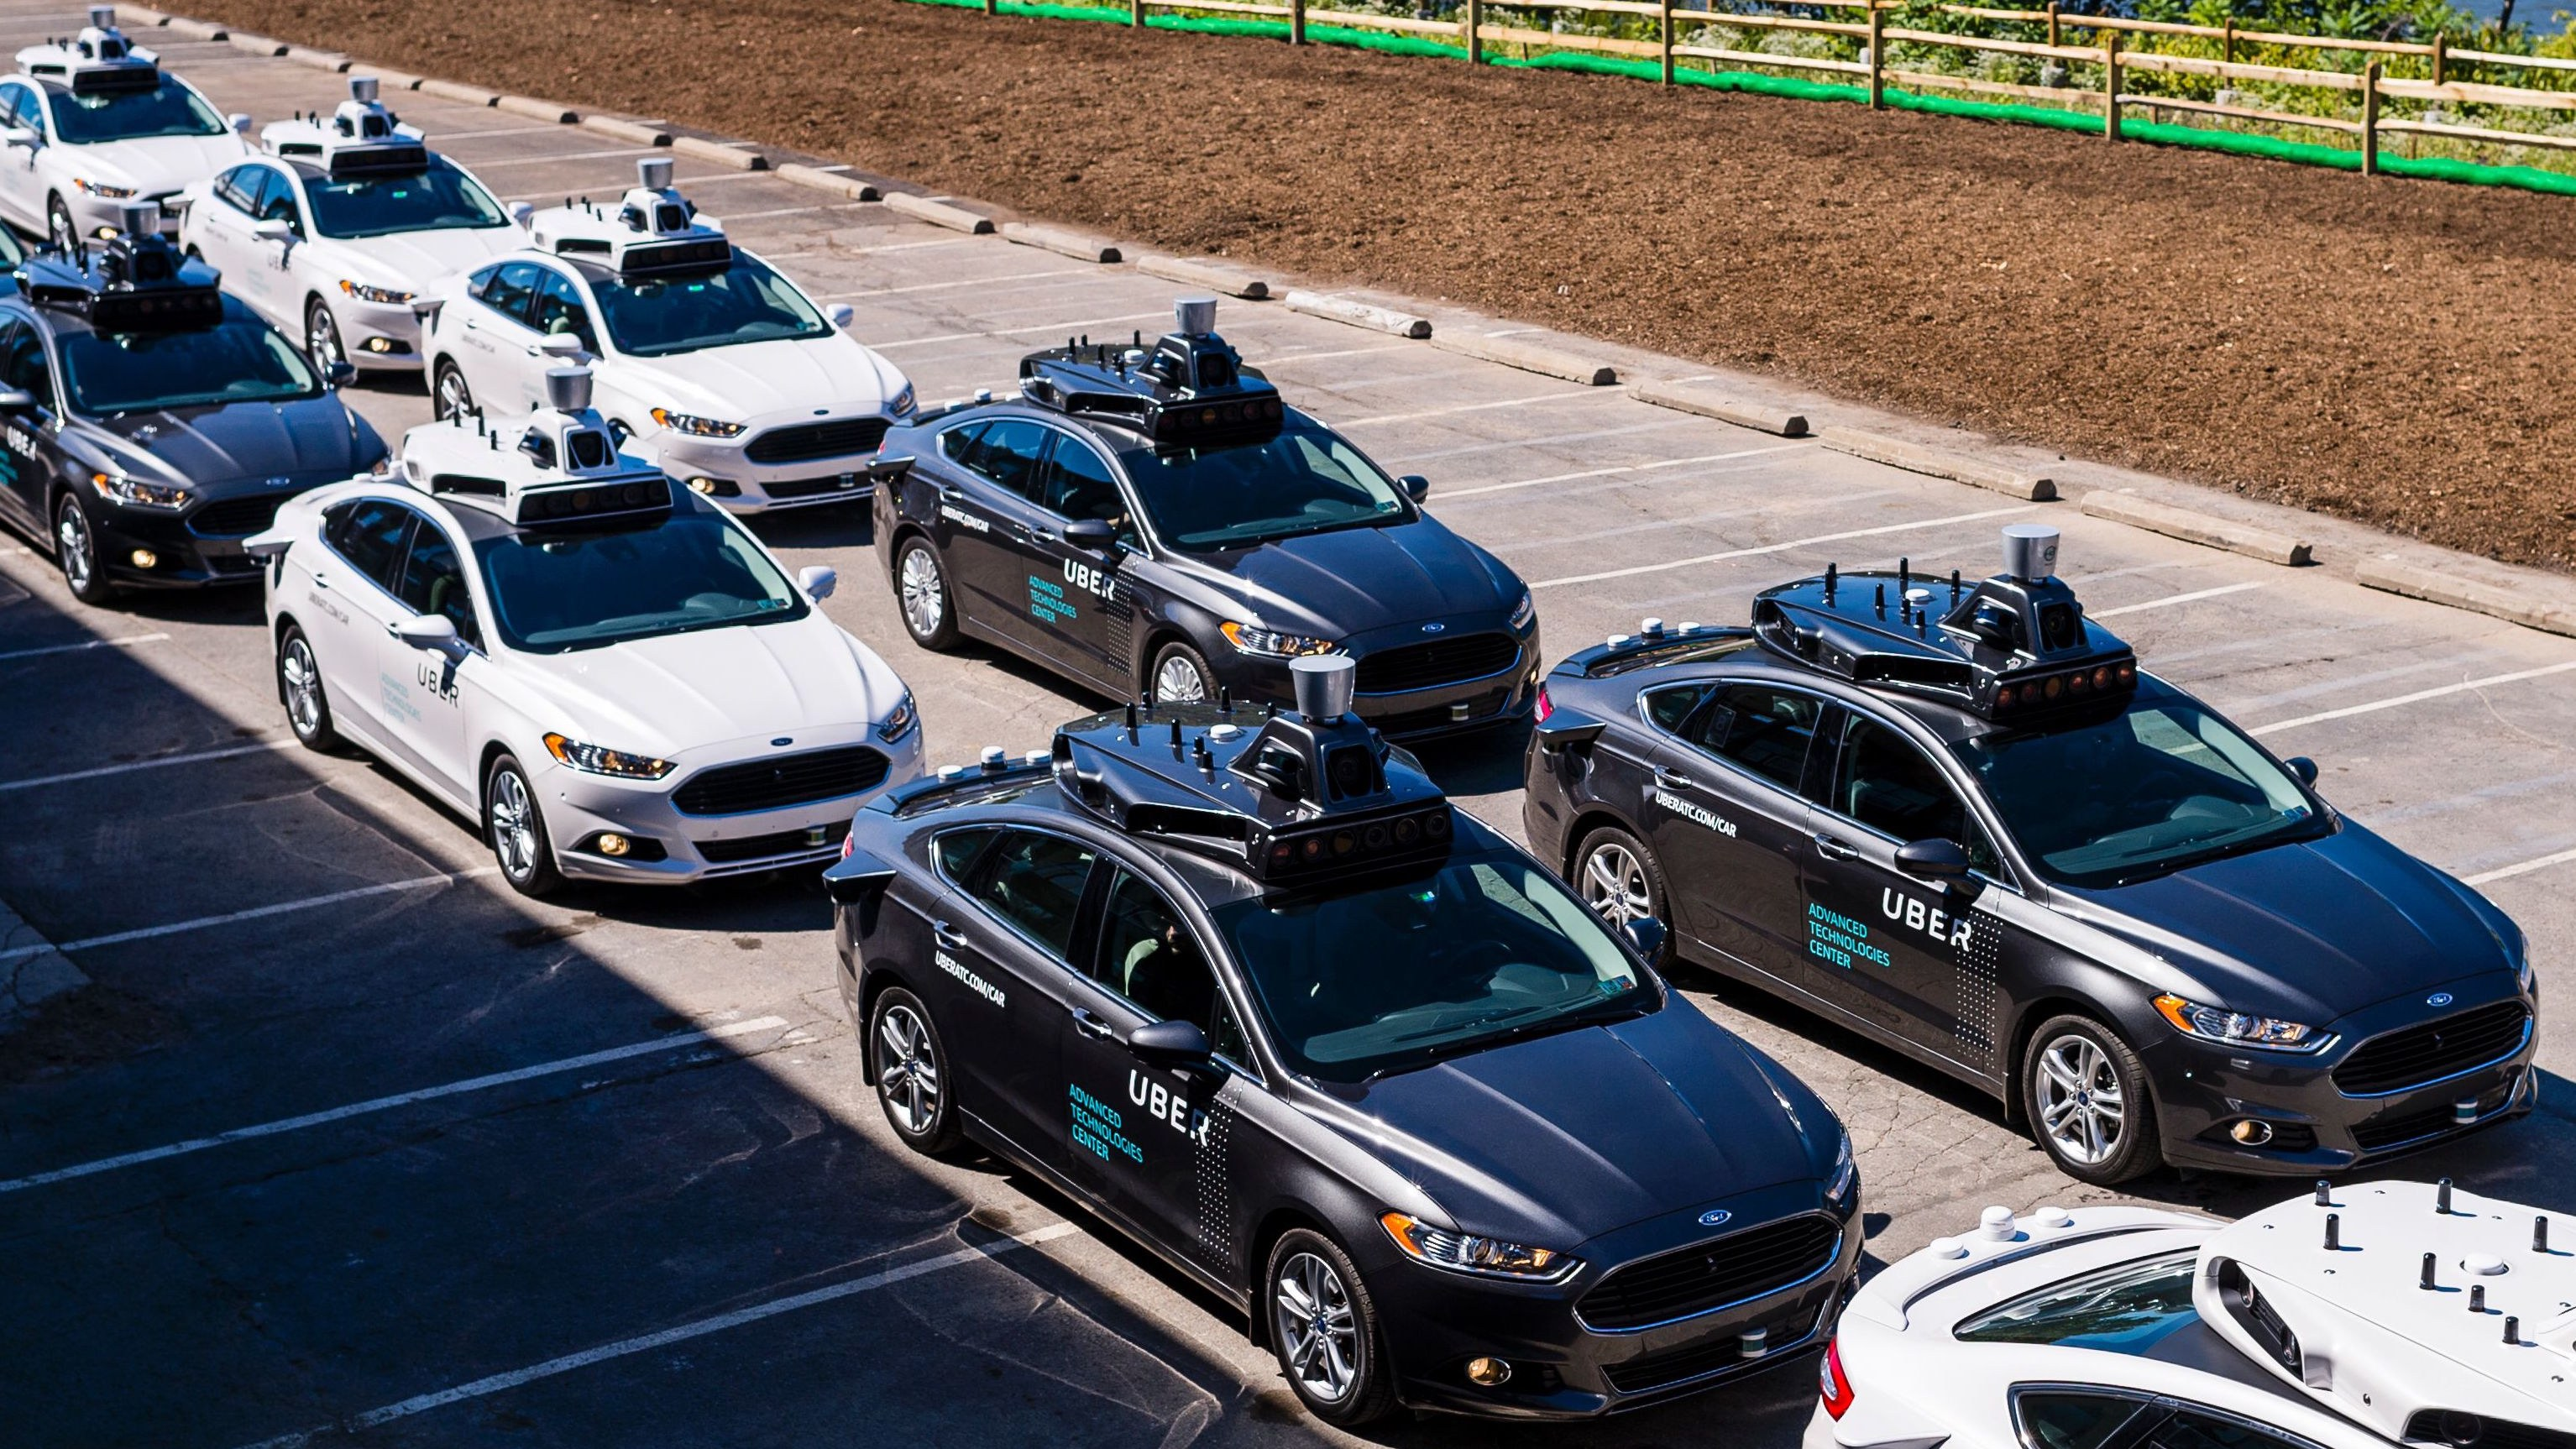
\includegraphics[width=0.19\textwidth]{uber.jpg} 
    \hspace{-0.25cm}
        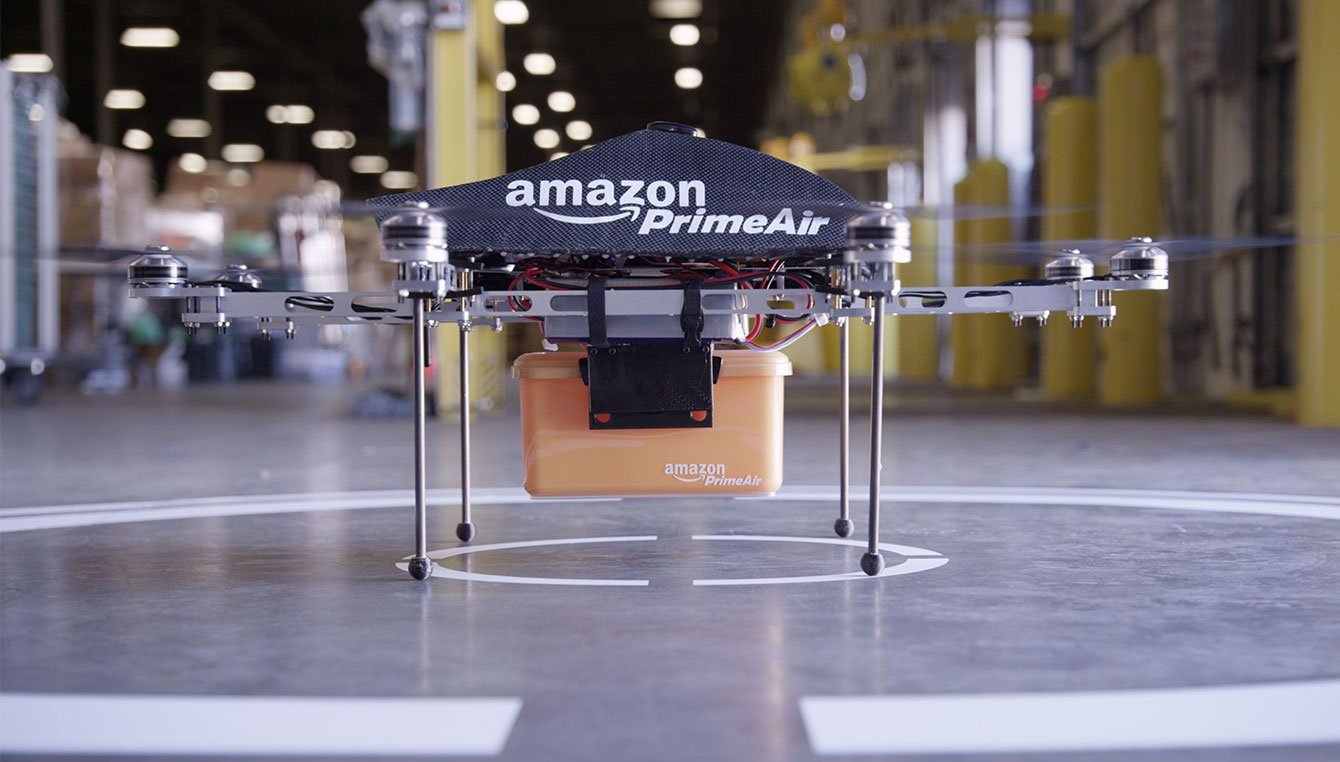
\includegraphics[width=0.19\textwidth]{amazon_delivery.jpg} 
    \hspace{-0.25cm}
        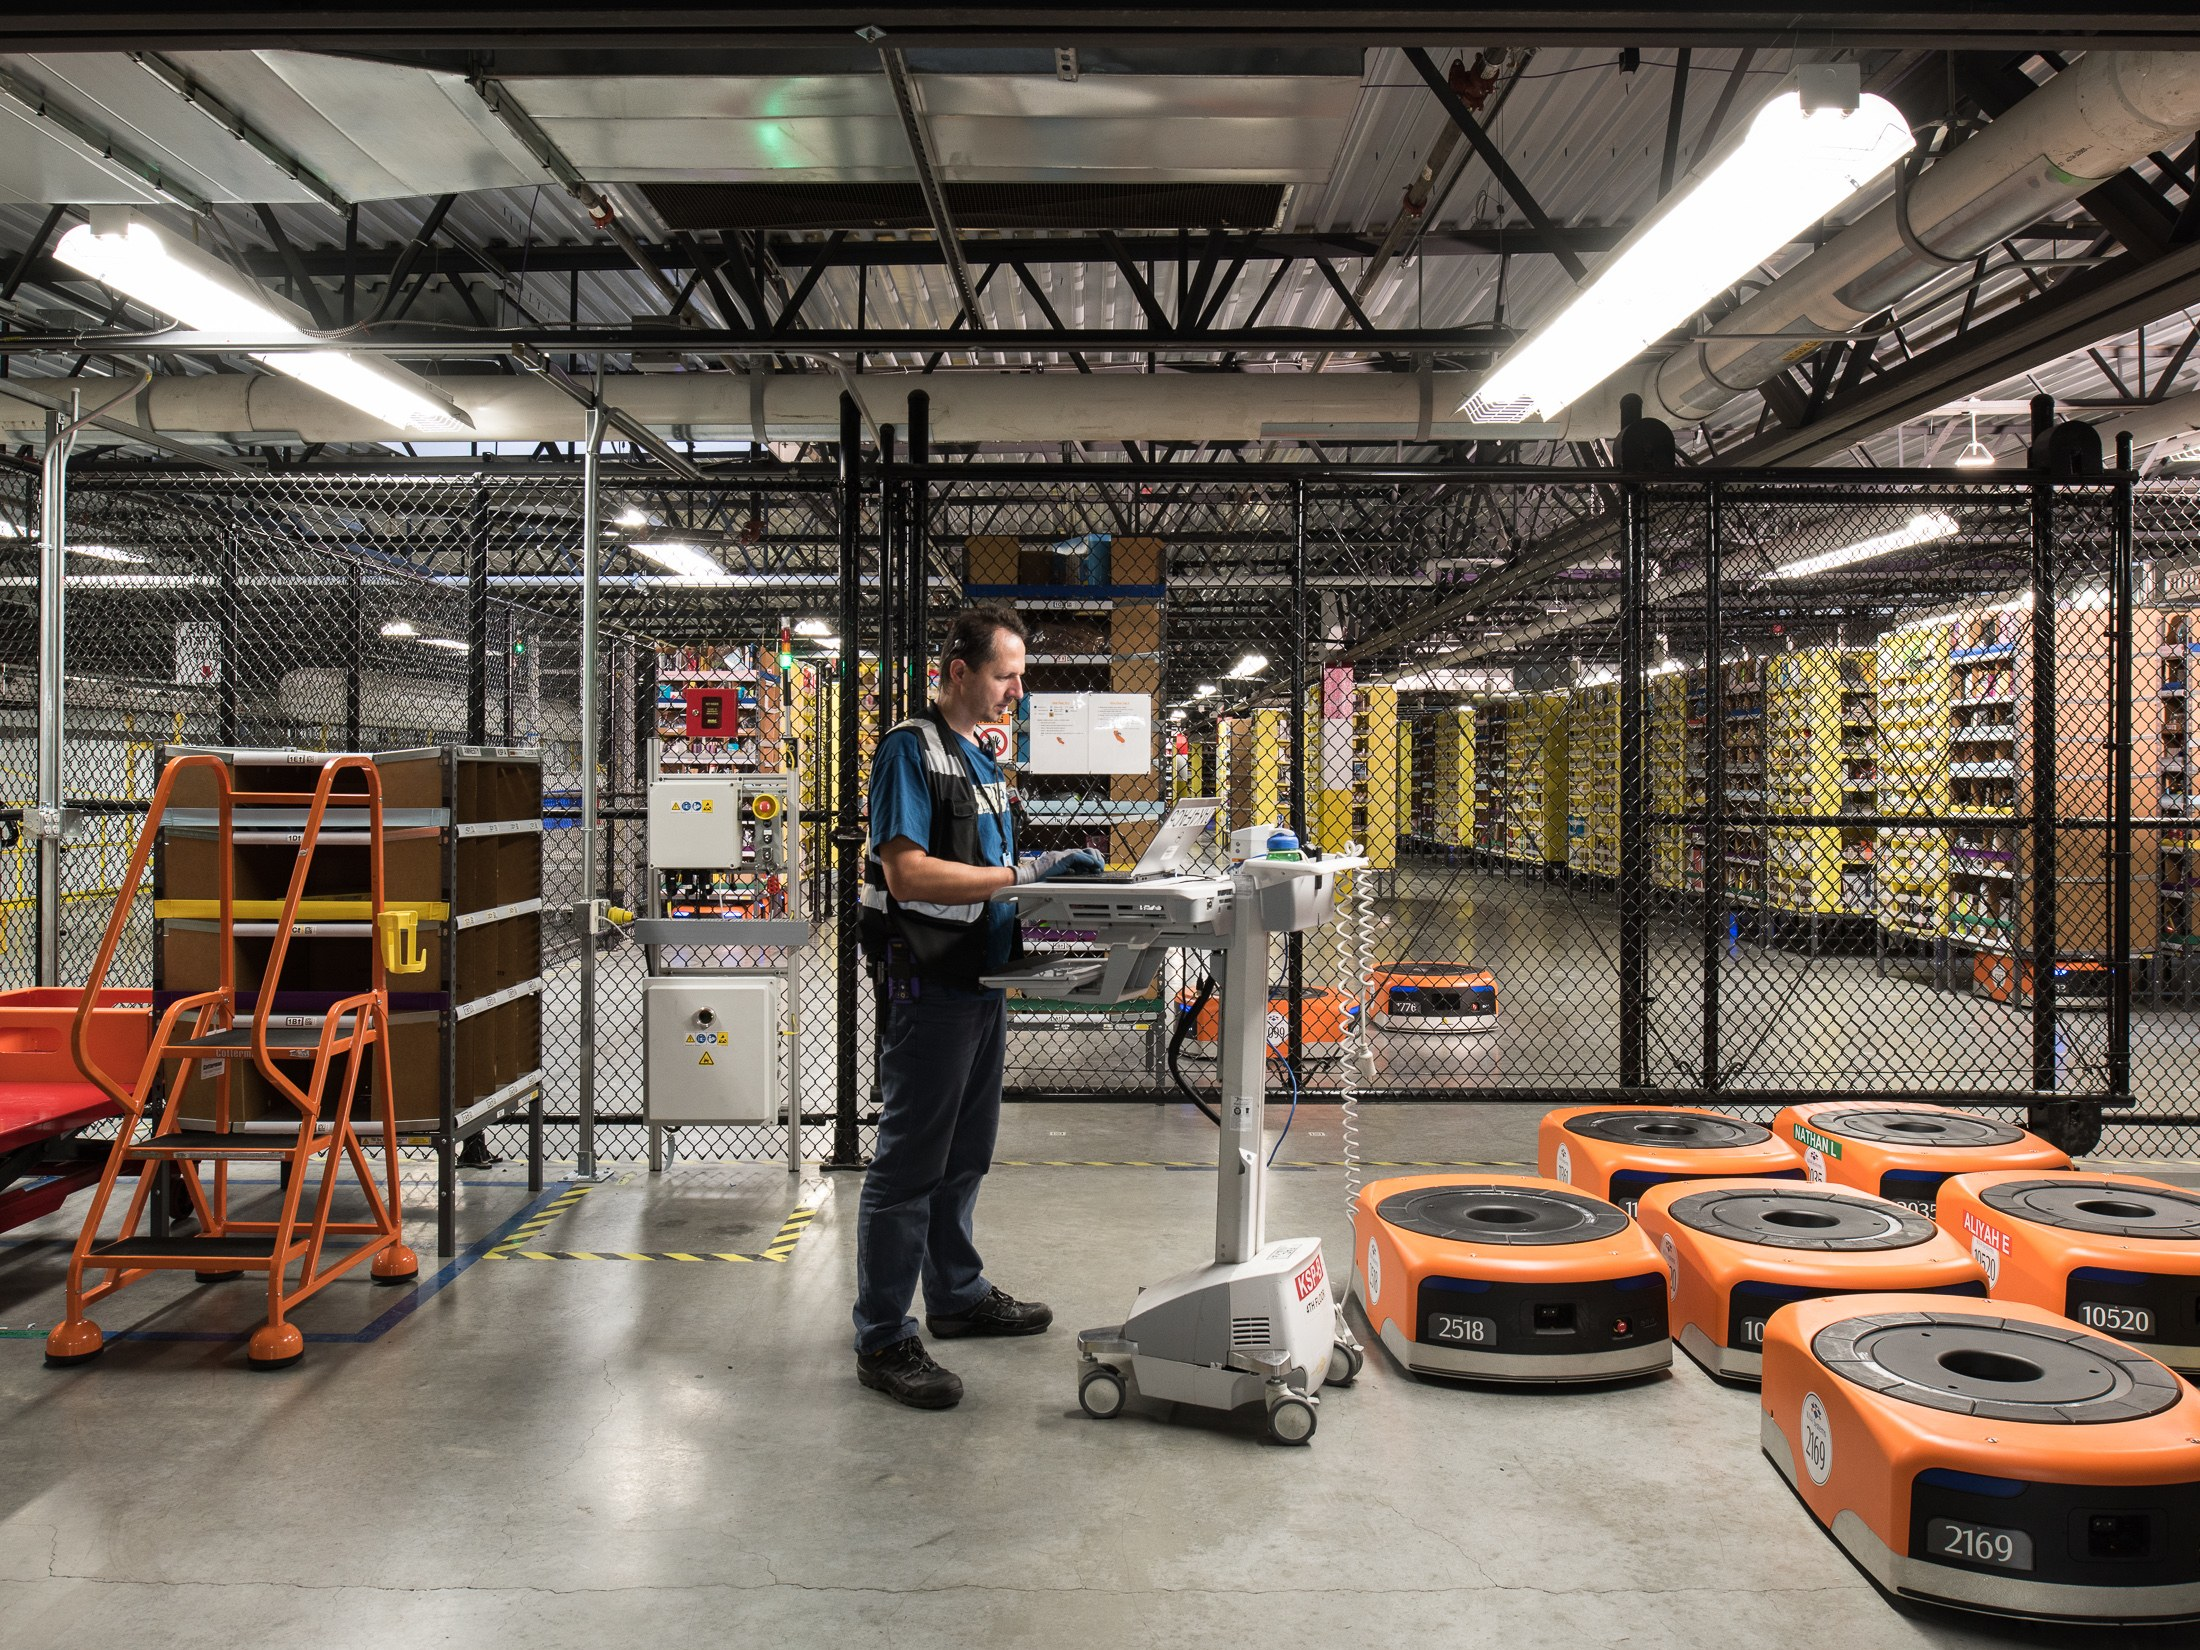
\includegraphics[width=0.145\textwidth]{kiva.jpg} 
    \hspace{-0.25cm}
        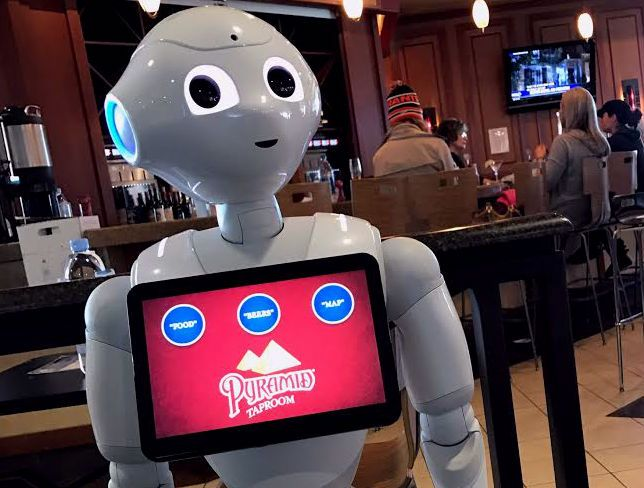
\includegraphics[width=0.145\textwidth]{Pepper.jpg} 
    \hspace{-0.25cm}
    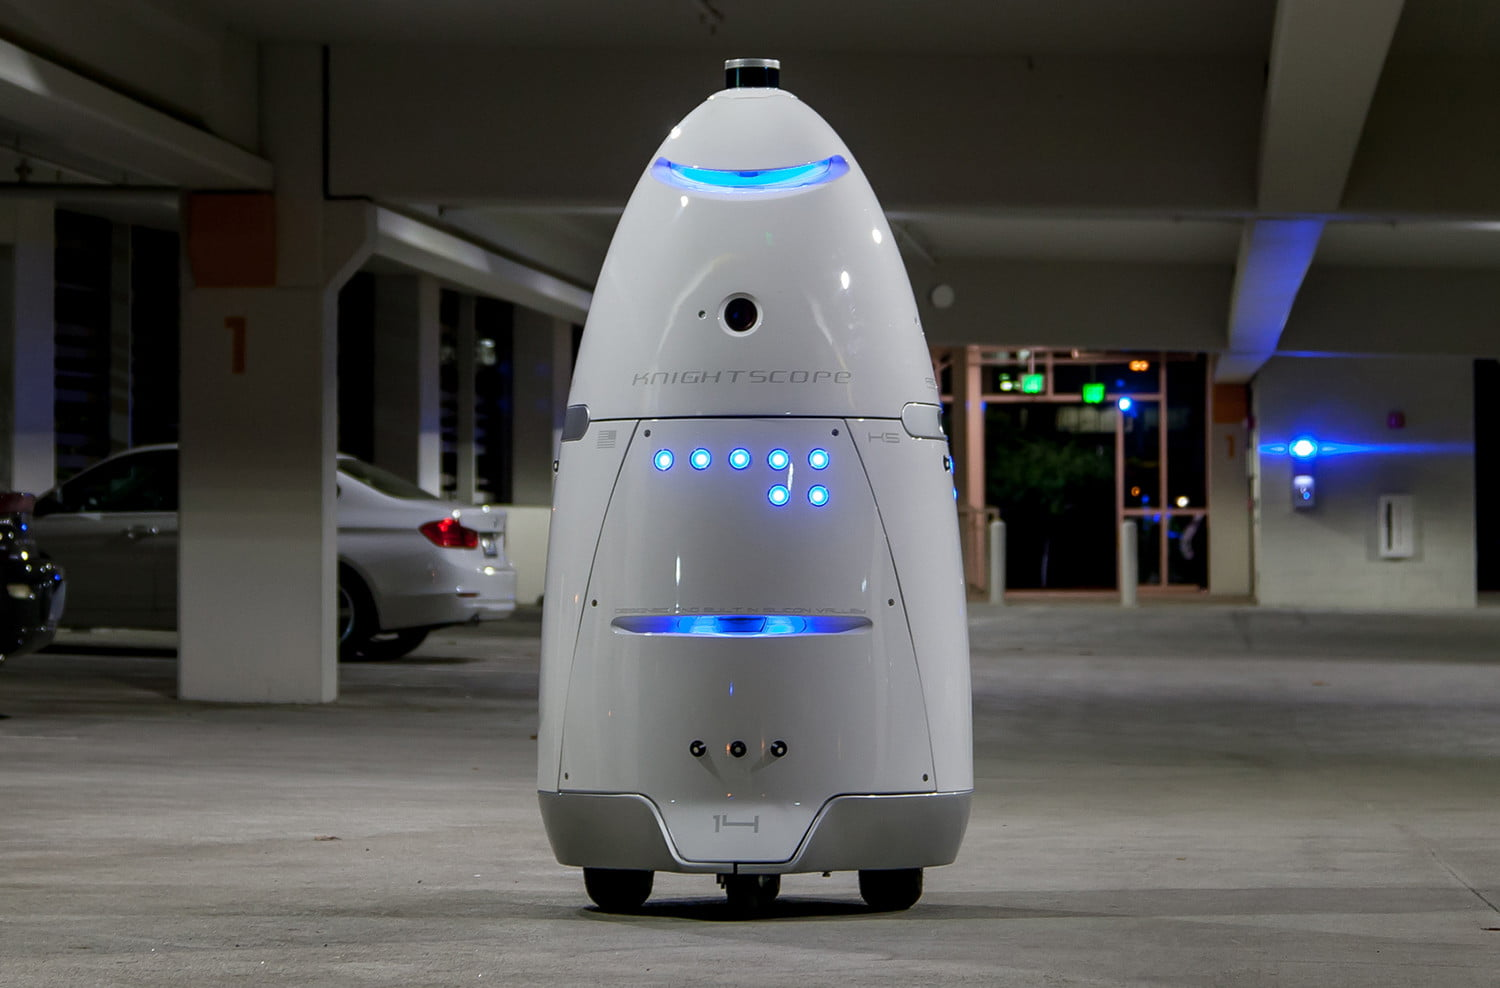
\includegraphics[width=0.17\textwidth]{knightscope.jpg} 
    \hspace{-0.25cm}

    \caption{Autonomous robots for human environments, from left to right: Uber's self-driving car, Amazon's delivery drone, Amazon's Kiva warehouse robot, SoftBank's Pepper advertising a restaurant, Knightscope's security robot}
    \label{fig:robots}
\end{figure*}

What distinguishes many of these projects from previous generations is the explicit desire to integrate robots en masse into human environments, rather than contain them to labs or factories. There are obvious advantages to being able to make use of spaces not specially prepared for robots, opening up larger swaths of the world including the outdoors for operation and more tasks that can be automated and commercialized. Just as obvious are the challenges, and while some are simply more advanced forms of previous technical questions in autonomy research (e.g. localization without support infrastructure), the social challenge of having to at least coexist with humans adds a whole new dimension to the autonomy problem.


It is this new dimension that concerns us. Autonomous robotics research and human-robot interaction have existed side-by-side as separate fields of research for decades, but the creation of integrated human-robot environments brings both subjects into contact. In such spaces it may not even be meaningful to think of the two subjects as neatly separable, if autonomy cannot be achieved while ignoring nearby humans as someone else's problem. What new research paradigm will we need to make this fusion successful?

This report will investigate the convergence of robot autonomy research and human-robot interaction research in the literature. We will examine major works and goals of both fields that reveal common ground useful to the development of integrated human-robot environments. In particular, we will look to develop our own theory about the new approach these environments will call for, and find what evidence exists to support further studies into the nature of the autonomous, human-compliant robot.

Our investigation is divided into two major chapters covering each of our main subjects, followed by a discussion and conclusion chapter to summarize our findings. First, however, we will take a closer look at existing theory surrounding the integration of humans and robots.




%Three Engineers, Hundreds of Robots, One Warehouse (Kiva 2008 example)
%https://spectrum.ieee.org/robotics/robotics-software/three-engineers-hundreds-of-robots-one-warehouse

%The cocktail party robot: Sound source separation and localisation with an active binaural head

%The strands project: Long-term autonomy in everyday environments

%Autofac



\section{Background}

%compliance/consent takes place not just on the part of the robot, but the human

Before we begin surveying research in autonomy and human-robot interaction, we should expand on the intuition that motivated this investigation. We have raised the idea that autonomous robotics in human spaces warrants special scrutiny by acknowledging products, business investment and academic attention, but not what is actually challenging about an independent robot operating among us over operating in a controlled space. Why should we need a new perspective for autonomy in human environments?

Setting aside the purely technical difficulties of less-structured spaces and uninstrumented users, part of our intuition comes from the public's own apprehensive reaction to this research. Self-driving car companies are extremely sensitive to the perception of safety issues surrounding their work - a single death in testing was enough for Uber to suspend its autonomous car testing entirely~\footnote{https://www.usatoday.com/story/opinion/nation-now/2018/06/25/uber-self-driving-car-death-blame-human-driver-column/730754002/}. Robots are not brought into Amazon's warehouses to support human workers, but to obsolete them, and the fear of automation of labor stalks every new application~\footnote{https://www.technologyreview.com/the-download/609672/amazons-investment-in-robots-is-eliminating-human-jobs/}. Popular fiction is awash with examples of robots entering society as part of a decline into dystopia, such as the enslaved replicants of \textit{Blade Runner}, stoking the public's fear that such technology is meant to oppress or replace them rather than improve their lives.

%The why don't they use my robot paper?


%The Uber death
%Blade Runner
%https://www.technologyreview.com/the-download/609672/amazons-investment-in-robots-is-eliminating-human-jobs/ (The Amazon job-loss article)


Anxiety over the impact of automation is nothing new. The 1955 story \textit{Autofac}~\cite{dick1955autofac} introduced the idea of a "lights-off" factory, so thoroughly automated that it would not even need to be lit on the inside, and also posited a dystopian future where such factories escaped human control and threaten civilization. Science fiction's cautionary tales have not slowed down Amazon's picker challenge, where teams compete to replace the remaining human-completed tasks in Amazon's warehouses. If the Luddites did not stop the adoption of the Spinning Jenny, what obstacle does public apprehension toward autonomous robots present now?

What differentiates the creation of integrated human-robot environments from these other more general automation concerns is the personal proximity of the robot interaction. Even the most passive robot, by its presence, confronts bystanders with its existence, and exercising its autonomy may demand much more than that of them, as we shall discus below. Encounters with robots can now happen in the wild, unsupervised, whether or not an individual human might want anything to do with them. In essence, we are asking society at large to accept integration with robot agents, to normalize their presence in the workplace, the street and the home and acknowledge their right to share these spaces.

This acceptance is not a purely rhetorical matter. The concept of right-of-way, for example, is integral to functional navigation in society. Whether subways, buses, elevators or simple doorways, navigating human spaces means constantly engaging and cooperating with other agents trying to do the same thing, with only social custom as enforcement. There may be danger in assuming that these customs will naturally extend to robots, even the possibility of causing offense through presumption.

On their website, the Campaign to Stop Killer Robots~\footnote{https://www.stopkillerrobots.org/the-problem/} states that "Allowing life or death decisions to be made by machines crosses a fundamental moral line. Autonomous robots would lack human judgment and the ability to understand context." While said in the context of promoting a ban on autonomous weapon systems, the line between the life-or-death decisions a robotic soldier might make and those of say, a self-driving car, is not immediately clear. The Campaign represents a broad coalition of NGOs and experts with the goal of trying to avert a potential arms race before it begins, but other campaigns could rise up just as easily to oppose other goals of autonomy research, or the very idea of robot autonomy.

%https://www.stopkillerrobots.org/the-problem/

These intuitions surrounding the larger societal forces engaged by the creation of integrated human-robot environments must be organized to something cogent if they are to guide our literature review. To that end, we will begin this report by developing our theory of why the study of robot autonomy and human-robot interaction together presents unique and emergent problems that must be approached from a new perspective, supporting ourselves with background material that has considered these high-level problems.

\begin{figure*}
    \centering
    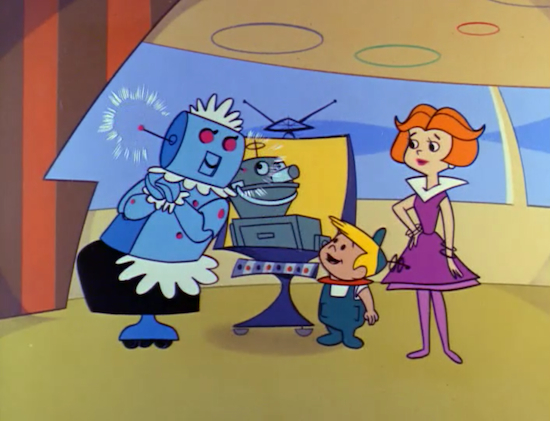
\includegraphics[width=0.47\textwidth]{jetsons.jpg} 
   % \hspace{-0.25cm}

    \caption{The animated future of \textit{The Jetsons}, where autonomous robots wait on the family's every need.}
    \label{fig:jetsons}
\end{figure*}

%premise 1
We already have our first premise - \textbf{there is a desire for autonomous robots that can operate in human environments}. This vision of robots for the home, the workplace and the public has permeated our expectations of the future since at least \textit{The Jetsons}(Figure~\ref{fig:jetsons}). The next generation of autonomous robots, whether cars, advertisers, cleaners, couriers, security and so on, distinguishes itself by moving into uncontrolled spaces where both direct and indirect interaction with humans is inevitable. This motivates our investigation into what autonomous operation in these newly integrated environments will require, particularly from the humans being asked to share these spaces.

\subsection{The Meaning of Autonomy}

Our first concern should be better understanding the definition of autonomy, beyond the loose similarity of a number of upcoming robot products. In \textit{Autonomy in Robots and Other Agents}~\cite{smithers1997autonomy}, Smithers criticizes what he sees as the vague and inconsistent use of the term autonomy in computer science and robotics when compared to other fields, such as biology, law, philosophy and so on. In these areas, autonomy is tied strongly to the concept of self-identity and "self-law-making", a layer of actualization that goes beyond the mere self-regulating controllers found in existing robotic systems. 

This disconnect between theoretical definitions of autonomy also plays out within the field of practical research. In \textit{Elephants Don't Play Chess}~\cite{brooks1990elephants}, Brooks notes that the thrust of AI research concerned with logical reasoning as the path to true general intelligence ignores that the development of such intelligence in living beings did not run through this route - in essence, that while a computer might beat an elephant at chess, we would consider the elephant much closer to us in terms of intelligence.

\begin{figure*}[!b]
    \centering
    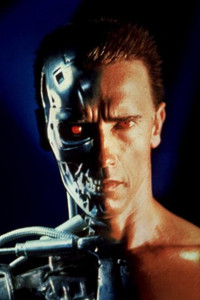
\includegraphics[width=0.35\textwidth]{terminator.png} 
   % \hspace{-0.25cm}

    \caption{The Terminator, which leverages its autonomy to terrify the audience.}
    \label{fig:terminator}
\end{figure*}

These critiques encourage the development of theories for robot autonomy that are grounded in actionable, recognizable principles. In \textit{Building "Fungus Eaters": Design Principles of Autonomous Agents}~\cite{pfeifer1996building}, Pfeifer presents a very different approach to intelligence and autonomy than classical AI, building from the ground up through the basics of what a lonely robot adrift on an alien world would need to survive - a "fungus eater", sustaining itself on forage and exploration. Pfeifer's principles outline self-sufficiency and the means to maintain it as the starting point for autonomy. The fungus-eater must be able to keep finding fungus to stay alive.



For an infamous example of robot autonomy recognizable to most audiences, consider the Terminator of the film franchise by the same name (Figure~\ref{fig:terminator}). The character's appeal as a villain is not just its durability and terrifying violence, but its ingenuity at navigating human society and pursuing its mission.

%Premise 2
Exploring the definition of autonomy leads to our second premise - \textbf{in order to be autonomous these robots will have to be intelligent and independent agents}. Independence here captures the self-sufficiency of Pfeifer, while intelligence covers the computational means to satisfy these needs, and agent the (likely embodied) notion of individual identity. What exact material conditions satisfy this definition will vary based on the robot's particular context (the fungus-eater is only autonomous on a world with fungus, after all), but any robot that does not satisfy our intuition concerning these properties is unlikely to be autonomous.

\subsection{Limitations of Social Recognition for Autonomous Robots}

If our autonomous robots are intelligent, independent agents like humans, then surely assimilation into human environments should be automatic so long as robots obey the social customs? Perhaps not - in \textit{Ants don't have Friends - Thoughts on Socially Intelligent Agents}~\cite{dautenhahn1997ants}, Dautenhan observes a divide in agent-based research, the product of its piecemeal pursuit through various fields. Artificial agents, including robots, are usually considered as clockwork automatons. They play their roles within a constructed system, and any deviation from proscribed behaviours is seen as a defect. Outside of their role in the agent-based system the artificial agent does not exist. Organic agents, particularly humans, are seen as holistic wholes, with additional layers of sociability, relationships and emotions underpinning their actions that extend beyond their current role. This disconnect means artificial and organic agents cannot simply be substituted one for the other, as they are not alike.

The social separation between human and artificial agents need not be a categorical one. In \textit{Mixing human and non-humans together: The sociology of a door closer}~\cite{johnson1988mixing}, Johnson notes that sociology does not have to limit itself to social relations between humans, or even between living beings - any entity that can hold up any sort of relation to another can be a site of sociological study, even a humble door-closing mechanism. Certainly the human tendency to anthropomorphize an unreliable car or a fond old tool should be familiar to most. In \textit{A Cyborg Manifesto}~\cite{haraway1991cyborg}, Haraway expounds at length that the 20th century had breached all conceptual barriers between man and animal, or man and machine, spreading the notion that we are all just physical constructs of varying complexity.

Robots would hardly even represent the first such artificial intelligent agents produced by humanity and socially integrated with us. In \textit{An Existing Ecologically Successful Genus of Collectively Intelligent Artificial Creatures}~\cite{kuipers2012existing}, Kuipers posits that corporations already represent an ecosystem of beings that live, die, feed, reproduce, interact, dominate and anything else we might attribute to life ("Corporations are people," to quote the 2012 Republican Presidential Nominee Mitt Romney). That the concept of a "good corporate citizen" is given any weight in public discourse makes the idea of a robot citizen light work by comparison.

\begin{figure*}
    \centering
    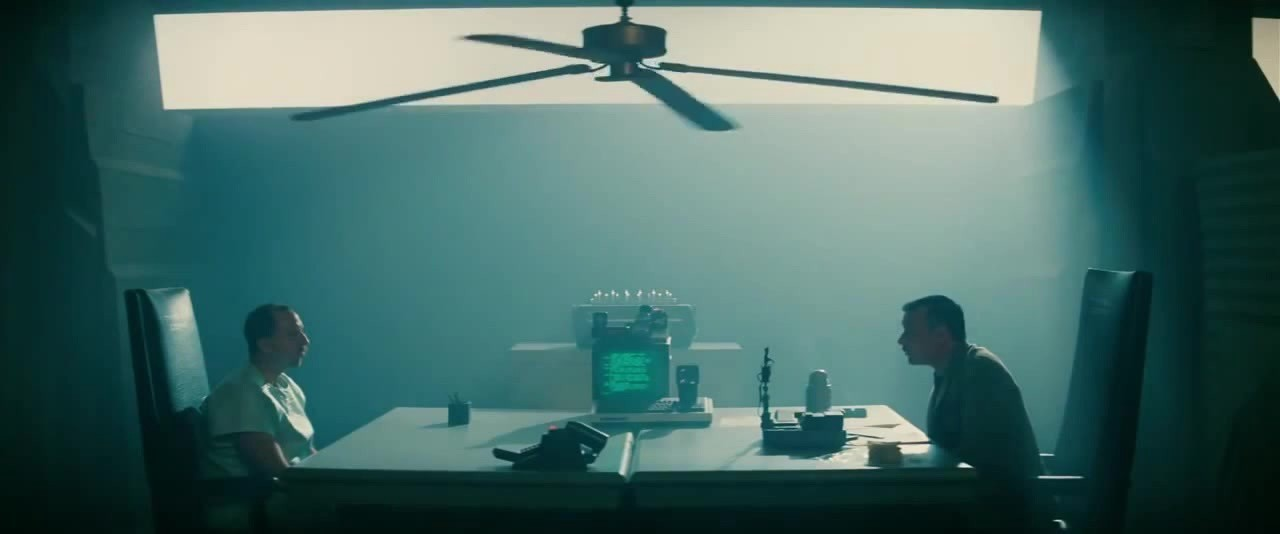
\includegraphics[width=0.7\textwidth]{voight.jpg} 
   % \hspace{-0.25cm}

    \caption{The Voight-Kampff test, the only way to separate a human from an artificial "replicant" in the movie \textit{Blade Runner}}
    \label{fig:voight}
\end{figure*}

Popular culture frequently explores our fascination with artificial personhood. In the film \textit{Blade Runner}, synthetic beings have become so human-like it takes a trained expert conducting the Voight-Kampff test to distinguish between them, yet this distinction makes the difference between a free-willed human and an enslaved "replicant" (Figure~\ref{fig:voight}). 

So if the distinction between human and robotic agents is limiting their ability to integrate with one another but no absolute separation is to blame, what is the problem? In \textit{When are robots intelligent autonomous agents?}~\cite{steels1995robots}, Steels argues that many more academic standards of intelligence used in the field are insufficiently persuasive for general use. In describing agents, he notes the notion of self-interest and self-maintenance as motivation for an agent's actions is key - a human travel agent, for example, does their work in return for compensation. They have a sense of personal agency that extends beyond the boundaries of their immediate role. Steels concludes that by his more exacting standard, no robot has yet become intelligent or autonomous.

%Tackling each component of intelligence, autonomy and agency separately, Steels concludes an agent must be self-sustaining and self-motivated - that it must have a grounded understanding of what it needs to succeed, and through its intelligence have a reasonable chance of obtaining it.



This leads us to our third premise - \textbf{humans perceive their agency as different from robots}. Even when a robot is self-sufficient and intelligent, it is typically only adapted to the role it was designed for, with no evidence of a larger existence outside of that context. Human agents, meanwhile, only play a part they are given, their agency is tied to their life and transcends temporary roles. Robot autonomy in the long-term and in human environments may introduce the idea that a robot must self-maintain, but not that a robot possesses true self-interest. Unlike us, a robot can never be said to act on its own behalf.

\subsection{The Significance of Social Agency}

\begin{figure*}[!b]
    \centering
    
\includegraphics[width=0.7\textwidth]{walle.jpg} 
   % \hspace{-0.25cm}

    \caption{The climactic moment in the film WALL-E, centered around signalling the survival of a robot's identity through a single intentional action.}
    \label{fig:walle}
\end{figure*}

What are the practical consequences of differentiating between human and robot agency? In \textit{How to build robots that make friends and influence people}~\cite{breazeal1999build}, Breazeal articulates the problem plainly - that in order to integrate human and robot society, humans must believe in the intentionality of their robot interlocutors. Robots must have identities as individuals, agents in their own right and possessing their own motivations and purposes that explain their actions, because these are the signifiers that humans use to recognize a fellow social agent. This does not require full equality to humans, or even perhaps that that this "intentionality" be "real" (for what value we give that term), but without the belief in it, a human cannot sustain a social relationship with a robot, and so any system within society that depends on that social connection will fail.

%So long as their agency is recognized, autonomous robots would afford unprecedented opportunities to transcend the limits of human nature in social contexts. The Principal-Agent problem, for example, when an actor of some kind struggles to align a proxy's self-interest with their own, or the Collective Action Problem, where all members of the group would benefit if only someone would volunteer for some unpleasant task their individual self-interest keeps them from. Tragedies of the Commons emerge when humans fail to regulate a shared resource amongst themselves and ruin it for everyone, but robots have no thoughts of greed or jealousy.

What would a socially-agentic robot look like? In \textit{Android arete: Toward a virtue ethic for computational agents}~\cite{coleman2001android}, Coleman proposes that while previous theories of computational ethics saw computers as tools through which other agents acted, soon they might be imagined as agents themselves, and therefore subject to their own moral obligations. If a robot cannot be the bearer of their own moral responsibilities then we cannot be said to be sharing society with them, merely with their developers or owners, whom robots at best represent remotely.

In the climax of the film \textit{WALL-E}, the eponymous robot closing his hand around that of his companion EVE demonstrates intentionality that signals to both EVE and the audience that WALL-E's identity and sense of self has survived (Figure~\ref{fig:walle}). No sophisticated framework or conscious explanation is needed, children and adults alike instinctively grasp the significance of this simple act of recognition.


We now have our fourth premise - \textbf{social agency requires the mutual recognition of and respect for each other's intentionality}. If robot autonomy does not assert a sense of identity and intent that humans can recognize, then they can never accept the robot as a social being capable of mutual recognition and reciprocation as another human or even an animal might. Without this crucial anchor, sincere social integration becomes impossible.

From the collected premises of our exploration, a hypothesis emerges. To review:

1) There is a desire for autonomous robots that can operate in human environments

2) In order to be autonomous these robots will have to be intelligent and independent agents

3) Humans perceive their agency as different from robots

4) Social agency requires the mutual recognition of and respect for each other's intentionality

\textbf{Therefore, the advancement of long-term robot autonomy in human environments will eventually require developing robot social agency.}

\subsection{History of the Robot Social Agency Motive}

Our hypothesis is not the first assertion of social agency for artificial beings. Alan Turing, in his momentous paper \textit{Computing Machinery and Intelligence}~\cite{turing2009computing}, presents a rhetorical case for the equivalence of computational and human agents once computers reach a recognizable level of human-like intelligence based on an "imitation game" (later known as the Turing Test) where if an examiner could not tell the difference between a human and a computer in a text conversation, the distinction between the two becomes moot, and all the agency we would attribute to one should be extended to both. 

As on many other topics, Turing's views on artificial intelligence had a lasting impact on the field, and shades of these sentiments can be found underpinning many of the works we have already considered, whether Breazeal's exploration of intentionality for robots, Haraway erasing the line between man and machine through the cyborg, or Coleman's investiture of moral weight to the robotic coworker. Certainly popular culture has a fascination with exploring synthetic personhood, so it cannot be said that social agency for robots is an unexplored idea.

What distinguishes our own formulation of the issue is its deceptively narrow scope and grounding in definite, ongoing research and market activity. These are not the hypothetical human-equal agents of Turing's conjecture or popular imagination, but tentative half-steps into social environments that businesses and labs are already in the process of making, with practical performance and commercial motives rather than high-minded philosophical ones. Our concern is not simply if agency and autonomy are connected in the abstract, but whether the field's present efforts toward bringing robots to human environments can gain by such a connection.

Testing our hypothesis will help guide our survey for what supporting evidence it would need and where to look. We can begin to identify what behaviours researchers see as critical to a robot's autonomy and cross-reference them with relevant work in human-robot interaction on how those behaviours will be received by human society and what motivates those reactions. If our theory holds, we may uncover evidence that the success of one will depend on the other, and discover what conclusions researchers have already drawn about the nature of this relationship.

%12 entries

%Building "Fungus Eaters": Design Principles of Autonomous Agents	Rolf Pfeifer's work about what it takes to be autonomous. Good starting point to build toward what it takes to be autonomous among people.

%Elephants Don't Play Chess	Another important Rodney Brooks paper, part of the philosophy of embodied, modern AI over classical.

%Vehicles	Brietenberg, almost exclusively about our projections onto a machine of lifelike characteristics

%How to build robots that make friends and influence people	Immediately makes point that robots need to convey intentionality, that humans recognize them. Important to independent autonomy

%The Principal-Agent Problem

%Collective Action Problems

%Ants don't have Friends - Thoughts on Socially Intelligent Agents

%Autonomy in Robots and Other Agents (TIM SMITHERS)

%AN EXISTING, ECOLOGICALLY-SUCCESSFUL GENUS OF COLLECTIVELY INTELLIGENT ARTIFICIAL CREATURES

%Mixing human and non-humans togetehr: The sociology of a door closer

%Android arete: Toward a virtue ethic for computational agents

%When are robots intelligent autonomous agents?

%https://slate.com/technology/2018/04/i-judge-men-based-on-how-they-talk-to-the-amazon-echos-alexa.html

\chapter{Autonomy}

The first of our major areas of interest is robotic autonomy research. In \textit{Autonomous Agents: From Biological Inspiration to Implementation and Control}~\cite{bekey2005autonomous}, Bekey defines autonomous robots as "intelligent machines capable of performing tasks in the world by themselves, without explicit human control", a definition compatible with our earlier exploration of the idea. For our purposes, "pure" autonomy research will cover the fundamental requirements of an unsupervised and self-sustaining robot regardless of its specific duties or environment.

Increasing the autonomy of machines has been a foundational pursuit of robotics since its inception, partly through its close relationship with artificial intelligence research. In the post-war period, this tight coupling and the era of symbolic-logic-driven (or "Good Old Fashioned") AI produced Shakey~\cite{nilsson1984shakey}, an autonomous, mobile robot who for all its advances also demonstrated the limitations of the highly rational, abstract paradigm of robot AI. That paradigm would shift in the 80s toward a more "bottom-up", behaviour-driven approach heralded by the likes of Rodney Brooks' Subsumption Architecture~\cite{brooks1986robust} and later the book \textit{Probabilistic Robotics}~\cite{thrun2005probabilistic}. Now the ascendance of machine learning promises new models that can outperform the hand-crafted systems of yesteryear by discovering features and correlations too abstract for human developers.

The methods may change, but the goals remain largely the same: make robots more usefully independent, and for longer.



%Speaking Swarmish: Human-Robot Interface Design for Large Swarms of Autonomous Mobile Robots

%Designing interfaces for multi-user, multi-robot systems	Design principle study for mixed human-robot teams, useful when discussing autonomy	





%Speaking Swarmish: Human-Robot Interface Design for Large Swarms of Autonomous Mobile Robots

%Designing interfaces for multi-user, multi-robot systems	Design principle study for mixed human-robot teams, useful when discussing autonomy	

%Probabilistic robotics

%Autonomous Agents: From Biological Inspiration to Implementation and Control 

%Rodney Brooks subsumption architecture

%Shakey the Robot	It's Shakey! Just a good part of robotic history, important to reference while giving background


\section{Long-Term Autonomy}

Long-Term Autonomy (LTA) refers to those aspects of robot autonomy specifically concerned with keeping the robot autonomous through many interactions, ideally indefinitely. Our theory touched on the importance of prioritizing survival and self-interest as part of agency, and this may be the practical research area that best represents this.

\subsection{Recharge Behaviour}

Issues of autonomous recharging and energy management are a fundamental topic in LTA - without the ability to power itself, a robot must either depend on outside assistance or it will not survive in the long term. Certainly some of the most well-known autonomous robots, such as the Roomba, have held autonomous recharge as a critical feature. Willow Garage's PR2 robot and the research around it represented a notable effort in pursuit of that goal - in \textit{Long-Term Autonomy in Office Environments}~\cite{meeussen2011long} they studied how long their robot could keep up its hourly autonomous recharge behaviour with only occasional human support. That test lasted thirteen days and over a 100km of travel, setting a benchmark for how challenging keeping robots powered can be. Meanwhile, in \textit{Autonomous door opening and plugging in with a personal robot}~\cite{meeussen2010autonomous}, they examined the navigation difficulties of doorway traversal through an office to get back to a recharge point. In a world where robots may need to face stairs, locks, blocking pieces of furniture and uncooperative coworkers to reach the power they need, the number of obstacles to their survival can seem endless.

More investigations into autonomous recharging have been undertaken outside of Willow Garage. In \textit{Staying Alive Longer: Autonomous Robot Recharging Put To The Test}~\cite{silverman2003staying}, the adoption of a recharging mechanism is presented as a precondition for true long-term autonomy, and immediately turns their research robot into a 24-hour sentry for the lab. In \textit{Basic cycles, utility and opportunism in self-sufficient robots}~\cite{mcfarland1997basic}, this intuition is codified into an evaluative framework to assess the time and energy cost efficiency of different behaviours with different robots. The common thread of these projects and the Willow Garage work is clear - autonomy in the long term demands the robot be able to keep itself 'alive', pursuing survival alongside or above its other duties. 

%Autonomous door opening and plugging in with a personal robot	Combines door navigation with recharging task, which ties the activities together into LTA

%Staying Alive Longer: Autonomous Robot Charging Put To The Test

%Basic cycles, utility and opportunism in self-sufficient robots

%Long-Term Autonomy in Office Environments	A solid case-study of running a robot in a lab for two weeks, letting it recharge itself and seeing when it would need and request help

\subsection{Scheduling and Allocation}


Once a robot is operational, it must be put to work. Most robot research will consider a single task or interaction in isolation, but LTA research connects a variety of tasks a robot will perform over their lifespan. Task allocation is one topic connected to this area that touches on a wide variety of issues relevant to autonomous multi-robot groups. In \textit{A Comprehensive Taxonomy for Multi-Robot Task Allocation}~\cite{korsah2013comprehensive}, Korash argues most forms of work one might want to divide among a team of robots can be categorized according to four types of problem complexity, proposing generalized solutions that affect broad swaths of autonomous operation.

Some approaches to allocation solve the problem globally over all robots and distribute the solution, in the manner of a team coming together to work out a schedule. In {Fair subdivision of multi-robot tasks}~\cite{higuera2013fair}, for example, a central server connecting a heterogeneous group of robots works out solutions to match the available capabilities of different robots to the needs of different types of work. Meanwhile, in \textit{Multi-Robot Task Allocation in Uncertain Conditions}~\cite{gerkey2003multi}, the focus is on what allocations and strategies to choose when some features of the available tasks are ambiguous.

Allocation becomes more difficult when dealing with distributed autonomous robots without central control, requiring creative individual policies to generate the desired overall outcome. For example, in \textit{A Fast and Frugal Method for Team-Task Allocation in a Multi-Robot Transportation System}~\cite{wawerla2010fast}, robots carrying supplies from sources to sinks can distribute themselves according to the productivity of each source by implementing a simple measure of patience - the longer the wait, the more likely a robot is to give up and try another queue, eventually reaching equilibrium. This is comparable to how customers allocate themselves at supermarket checkout lanes, gravitating toward short and fast-moving queues to naturally increase the system's throughput with no communication or central control.

What all of these methods share is some notion of individuals working together and playing by the same rules with an eye toward some common good. Sometimes this cooperation comes in the form of explicit directions from a central source, while other times it is the emergent property of each agent's individual actions, following rules designed to interact well with one another. Any breakdown in this system - some agents refusing to work together, or even deliberately exploiting openings made by these rules - could have severe consequences for the autonomy of the agents involved. In controlled spaces this might be avoided, but human environments are anything but controlled.

%?Dynamic Task assignment in robot swarms

%?a formal analysis of task allocation

%?simple auction for task allocation




\subsection{Field Studies}

Studies play an important role in LTA research, whether months-long longitudinal ones or batteries of individual interactions. The feedback that live robot results provides to both design and evaluation is invaluable, and in the case of some longitudinal field studies represents the real results of final products.

To that end, the well-known Roomba robotic vacuum cleaners by iRobot have provided a simple, practical example of autonomous home robotics the average consumer is already familiar with. A number of studies have featured the Roomba, including \textit{Robots in the Wild: Understanding long-term use}~\cite{sung2009robots}, \textit{Lessons learned from robotic vacuum cleaners entering the home ecosystem}~\cite{vaussard2014lessons}, \textit{How Robot Products become Social Products: An Ethnographic study of cleaning in the home}~\cite{forlizzi2007robotic}, and \textit{Service Robots in the Domestic Environment: A Study of the Roomba Vacuum in the Home}~\cite{forlizzi2006service}. These example studies involved as few as three or as many as thirty robots, spanning one to six months, with methodologies ranging from interviews to competing hand-held vacuums to photo-journals of user cleaning experiences. What all four hold in common, however, is an explicit interest in assessing the robot's autonomy through the eyes of everyday users, measuring its' impact through how it affects their lives and alters their habits. It is a reminder that robots are not made autonomous simply for their own sake, where the goal of most autonomy research relates back in some way to making a robot more useful to us as a tool or product.

Some investigations will place a robot into a public environment to collect more natural data from a broad cross-section of real users. Museums are a good choice of venue for these studies, such as in \textit{The mobot museum robot installations: a five year experiment}~\cite{nourbakhsh2003mobot}, since they provide a known environment, regular crowds and a selection of simple, useful duties for the robot to perform. In the mobot case, four robots were deployed over five years over the course of three successive deployment iterations, with the authors concluding that the most useful insight into long-term autonomy gained by the experiment was that it was possible at all under public constraints. 

A notably different example would be \textit{Experiences with an Autonomous Robot Attending AAAI}~\cite{michaud2001experiences}, less a long-term study than a test, in this case describing one of several autonomous robots attempting to meet a challenge to register, navigate and present its own experience at the conference. While structured differently than the mobot example and the Roomba studies, all of these efforts present robot autonomy in human environments as a challenge of maintaining autonomy while coexisting with humans.

%?Life-Long Learning of daily Human Routine in Home Environments	Applying learning and adaptation to human behaviour, a good example of a long-term project adapting itself.

%?The Snackbot: Documenting the design of a robot for long-term human-robot interaction	LONG-TERM HRI! Not multi-robot and maybe a little bare-bones, but here's a good example!




%Robots in the Wild: Understanding long-term use	Longitudinal study of 30 households with Roombas, answering question of whether people keep using them when novelty wears off. Novelty wearing off is a big concern for long-term autonomy	

%Lessons learned from robotic vacuum cleaners entering the home ecosystem

%How Robot Products become Social Products: An Ethnographic study of cleaning in the home.	Study of how families adapted to the Roomba, possibly useful in discussing how people adapt to the presence of robots in their lives.	

%Service Robots in the Domestic Environment: A Study of the Roomba Vacuum in the Home	It's about the Roomba! It's obviously relevant! Ethnography on how users long-term get along with service robots in the home.	

%The mobot museum robot installations: a five year experiment

%Experiences with an Autonomous Robot Attending AAAI

%Life-Long Learning of daily Human Routine in Home Environments	Applying learning and adaptation to human behaviour, a good example of a long-term project adapting itself.

%The Snackbot: Documenting the design of a robot for long-term human-robot interaction	LONG-TERM HRI! Not multi-robot and maybe a little bare-bones, but here's a good example!









\section{Navigation}

Navigation is another fundamental, almost defining aspect of robot autonomy. While not all autonomous robots are mobile (a factory arm or a receptionist, for example), a mobile robot is likely more autonomous than an immobile one, and the field of autonomous work it might participate in is vastly expanded. It also plays a major role in our motivation for this survey, as it affords many opportunities for direct and indirect interactions with humans.






\subsection{Navigation Algorithms}

Purely theoretical algorithms make up the foundations of robot navigation, solving in abstract the questions of path planning and obstacle avoidance. The famous A* algorithm~\cite{hart1968formal} is not specific to robotics - in fact, it is a graph traversal algorithm with many other applications in computer science - but it is an example of one such generalized theory imported by robot planners. 

Transitioning from pure theory to practical, real-world navigation requires addressing the specific needs of robots - for example, the Dynamic Window Approach (DWA), articulated in \textit{The Dynamic Window Approach to Collision Avoidance}~\cite{fox1997dynamic}. This method incorporates the physical constraints of a robot in motion, such as turn rates, speed and acceleration, to produce trajectories better adapted to real conditions. The approach has found traction among robot enthusiasts, coming prepackaged in the popular open-source robot software ROS's~\cite{quigley2009ros} standard navigation stack.

Even more challenging is considering the dynamic parts of the environment. In \textit{Motion Planning in Dynamic Environments Using Velocity Obstacles}~\cite{fiorini1998motion}, the positions and velocities of other agents in the environment - velocity obstacles - are considered when making the robot's own plans about where to go to ensure they won't instigate a collision.

Some of the most sophisticated of these navigation methods will incorporate the dynamic obstacles' own agency, predicting how they will react to the robot's presence. \textit{Reciprocal velocity obstacles for real-time multi-agent navigation}~\cite{van2008reciprocal} extends the velocity obstacle to consider their mutual interest in avoiding collisions while maintaining efficiency, allowing agents to depend on one another to smooth their trajectories. Many extensions have been built off this work, such as \textit{Bravo: Biased reciprocal velocity obstacles break symmetry in dense robot populations}~\cite{sadat2012bravo}, which addresses a particular use-case of crowds of robots navigating from source to sink and how to improve the efficiency of outcomes by favouring those leaving sources over those arriving. 

We can observe how as pure navigation is refined toward something usable, the issue of how to handle other agents - other people - navigating in the same space looms larger and larger. The intuition that cooperation makes for mutually satisfactory outcomes is easy to satisfy when the controllers of every agent are specified by the developer. In \textit{A Decentralized Approach to Formation Maneuvers}~\cite{lawton2003decentralized}, for example, groups of robots can be made to adopt different useful formations without the need for direct control - robots are moving in a distributed, autonomous manner, but the overall result can be directed. This leads naturally to the question of how to gain the same benefits when some agents are not written by the developer.





% Do I need Behaviors for Robust Door Opening and Doorway Traversal with a Force-Sensing Mobile Manipulator		Pure doorway navigation


%A* paper the name's up there

%velocity obstacle paper the name's up there

%The Dynamic Window Approach to Collision Avoidance	That classic paper from the directed reading, influential on robot navigation for problems like getting through a door.	

%Reciprocal velocity obstacles for real-time multi-agent navigation

%Bravo: Biased reciprocal velocity obstacles break symmetry in dense robot populations

%Behaviors for Robust Door Opening and Doorway Traversal with a Force-Sensing Mobile Manipulator		Pure doorway navigation

%A Decentralized Approach to Formation Maneuvers

\subsection{Biological Inspiration}

It would be a glaring omission for those developing navigation for robots to ignore the largest pool of inspiration on this subject available - biological life. Humans and animals both provide a wealth of practical solutions to navigation problems, honed over millions of years of evolution.

They also provide many examples of how to cooperate and coordinate, sometimes on grand scales, while every individual remains distinct. In \textit{PLEdestrians: A Least-Effort Approach to Crowd Simulation}~\cite{guy2010pledestrians}, thousands of simulated agents recreate the natural dynamics of humans moving as a crowd, including features like lane formation and crowd compression. In further work from the same lab, \textit{Directing Crowd Simulations Using Navigation Fields}~\cite{patil2011directing}, this crowd simulation was upgraded to include field-based control mechanisms to shape the flow and direction of the simulated mass of human-like agents. The testing opportunities for simulated robot navigation controllers to interact with masses of humans without the need for large groups of volunteers are obvious, but the simulated crowd agents themselves can be a source of insight for how to blend in with a group.

These insights can be turned back around to provide the basis of controllers for real robots. In \textit{A navigation approach for robots in crowded urban areas}~\cite{kummerle2013navigation}, the robot's navigation mission covers kilometers of city ground, so the researchers embrace "pedestrian-like" behaviour as the goal of their system, recognizing the boundaries of sidewalks, traffic lights, and other urban navigation customs. Meanwhile, in \textit{Dynamic path planning adopting human navigation strategies for a domestic mobile robot}~\cite{yuan2010dynamic}, knowledge about human strategies for navigating their own home is leveraged to improve robot performance at the same task. In both cases, the route to a successful robot navigation controller runs through learning from how humans already navigate these environments.

This potential for insight is not limited to humans. In \textit{Reducing spatial interference in robot teams by local-investment aggression}~\cite{zuluaga2005reducing}, biological inspiration is taken from the animal world through the use of displays of aggression. In nature, it's common throughout the animal kingdom for two animals to resolve a dispute through a display of force rather than the risk of an actual fight. The same insight could be applied to navigating robots blocking each other's paths - the more committed robot would advance toward the less committed one, causing it to retreat and breaking a potential deadlock. 

In other cases, particularly swarm robotics, inspiration comes from the group behaviours of many animals together. Reynolds' Boids, a software simulation detailed in \textit{Flocks, herds and schools: A distributed behavioral model}~\cite{reynolds1987flocks}, is a widely-cited model for recreating the movements of flocks of birds, herds of beasts and schools of fish - or potentially robots meant to simulate these things. For example, in \textit{Self-organized flocking in mobile robot swarms}~\cite{turgut2008self}, where the tiny Kobots are made to travel in a group as one "super-organism", Reynolds' flocking model is cited as the origin for this brand of robot behaviour.

These examples suggest many autonomy researchers are already aware of the value of biological inspiration to solve difficult problems in pure robot autonomy. Moving out of the lab and into inhabited environments, however, the question remains whether "human-inspired" is the same as "human-compliant".

%PLEdestrians: A Least-Effort Approach to Crowd Simulation

%Directing Crowd Simulations Using Navigation Fields

%A navigation approach for robots in crowded urban areas

%Dynamic path planning adopting human navigation strategies for a domestic mobile robot

%Reducing spatial interference in robot teams by local-investment aggression

%Flocks, herds and schools: A distributed behavioral model

%Self-organized flocking in mobile robot swarms












\chapter{Human-Robot Interaction}

The other half of our investigation concerns research in Human-Robot Interaction, covering almost any activity involving both humans and robots in any conceivable configuration. This broad mandate allows HRI to draw from many other fields, such as human-computer interaction, the humanities, multi-agent theory, and of course autonomous robotics. Evidence for this breadth can be seen in \textit{Survey of metrics for human-robot interaction}~\cite{murphy2013survey} - while many other robotics fields might be satisfied with a small number of objective measures like efficiency or throughput, the survey authors found 42 different metrics in HRI, and the number may have grown in the last five years since that survey.

It would be remarkable if, given this broad range of investigation, many researchers in HRI had not already identified relations between their work and autonomy research. Finding such cases of explicit or implicit connection between what we observed in our previous chapter and the pursuits of the HRI field will motivate our survey here.









%?Timing in Multimodal turn-taking Interactions: Control and Analysis using Timed Petri Nets	HRI case dealing with turn-taking interaction styles.

%?Reasoning for a multi-modal service robot considering uncertainty in human-robot interactions	POMDPs, remember them from Joelle? A reasoning system to fill the gap between sensors/actuators and POMDPs, multi-modal fusion

%Survey of metrics for human-robot interaction	Thank goodness, a survey of dozens of methods to measure human-robot interaction.


\section{Human-Compliant Navigation}

While in the previous chapter we discussed examples of "pure" robotic navigation, focusing on the mechanics of getting from one point to another, some have addressed the additional layers of complexity added through contact with humans. Beyond simply being inspired by humans or modelling them in the abstract, this means considering whether the motions of the robot about its business will be satisfactory to the humans it encounters, and whether this will ultimately secure their compliance.

In \textit{Human-Aware Robot Navigation: A Survey}~\cite{kruse2013human}, the features of a "human-aware" navigation system are listed as human comfort, natural motion, and motion under social constraints, with additional consideration for the nuances of human crowds and formations as well as their propensity to learn and adapt. These are all features that emphasize the human as more than just a navigating agent, a "velocity obstacle". They capture the full breadth of their agency, marking the transition from the sparse definition of the term used within computer science to the full-bodied one humans apply to other humans.


%Human-Aware Navigation: A Survey	Similar to that social robotics paper, a survey and classification of this type of project



\subsection{Proxemics}

Our first stop when considering the human impact of robot navigation is as simple as testing how humans react to being near robots. In \textit{Evaluation of Passing Distance for Social Robots}~\cite{pacchierotti2006evaluation}, a user study gauging the range of comfortable distances for a robot to maintain while passing a human in the hall, made the expected observation that passing too close was displeasing to participants. However, it also found that passing too far - especially if done sharply, such as a robot at the far end of the hall abruptly hugging the wall - was similarly awkward. 

Relative positioning can also be thought of as a communication signal. In \textit{Toward Understanding Social Cues and Signals in Human-Robot Interaction: Effects of Robot Gaze and Proxemic Behaviour}~\cite{fiore2013toward}, distance was found to be more effective at signalling intent than visual gaze for human subjects passing in a corridor. That repeated interactions were found to solidify this signal also has implications for robot behaviour in the long-term, promoting consistency.

The distances and positioning modelled in proxemics have deeper implications than, say, the ideal emergency stop distance for a given robot obstacle avoider. In \textit{Human-Robot Proxemics: Physical and psychological distancing in human-robot interaction}~\cite{mumm2011human}, a study found a relationship between the likeability of the robot and the proximity the human felt comfortable maintaining. - and that this relationship was two-way, where an unwelcome gaze could drive a participant further away.

%Evaluation of Passing Distance for Social Robots	Another proxemic user study, interesting finding that too much lateral distance is also weird besides too little	

%Toward Understanding Social Cues and Signals in Human-Robot Interaction: Effects of Robot Gaze and Proxemic Behaviour	Corridor passing, proxemic was influential while gaze was not, multiple interactions were more effective	

%Human-Robot Proxemics: Physical and psychological distancing in human-robot interaction	Adapting social norms to maintaining distance between social interlocuters.

\subsection{Model-Based Navigation}

Proxemics might be considered as one example of model-based navigation, that is, navigation approaches that make use of explicitly-designed models of human behaviour and the developer's domain knowledge on the subject. These models would include many of the pedestrian-simulators we discussed previously under biologically-inspired navigation, with the goal of accurately recreating specifically-human behaviours. In \textit{A Predictive Collision Avoidance Model for Pedestrian Simulation}~\cite{karamouzas2009predictive}, the term "visually compelling" is used to describe the result, speaking to the viewer's own intuitive recognition of familiar crowd behaviour.

This leads to the \textit{Social Forces Model for Pedestrian Dynamics}~\cite{helbing1995social}, a hand-crafted model for explicitly describing the motion of humans in public spaces like malls. Robot controllers built on this model, such as the one described in \textit{Towards a socially acceptable collision avoidance for a mobile robot navigating among pedestrians using a pedestrian model}~\cite{shiomi2014towards}, find their success is enhanced beyond simple collision-avoidance approaches in pure navigation, as the more socially-compliant robot slots into human environments with a minimum of disruption.

This type of comparison between human-inspired models and more abstract, agent-based multi-agent navigation is explicitly investigated in \textit{Local reactive robot navigation: A comparison between reciprocal velocity obstacle variants and human-like behavior}~\cite{guzzi2013local}. When weighing reciprocal-velocity-obstacle approaches against human-inspired ones in simulation, considering safety and throughput, the authors found a human-like approach often outperformed the more abstract competitors.



%A Predictive Collision Avoidance Model for Pedestrian Simulation

%Towards a socially acceptable collision avoidance for a mobile robot navigating among pedestrians using a pedestrian model

%Local reactive robot navigation: A comparison between reciprocal velocity obstacle variants and human-like behavior 

%Social Forces Model for Pedestrian Dynamics




\subsection{Machine Learning}

Alternatively to model-building, machine learning offers new and increasingly competitive methods to capture the subtleties of human-compliant navigation. In \textit{Social LSTM: human trajectory prediction in crowded spaces}~\cite{alahi2016social}, we see a machine-learning based example of the previous crowd behaviour simulations that were based on hand-crafted rule-sets. Using videos of crowds and neural network techniques, the resultant system can predict the trajectories of pedestrians on video with comparable accuracy to the social forces model yet with none of the explicit, laborious modelling. 

This is not meant to imply that machine learning is blind to insight or domain knowledge. In \textit{Learning social etiquette: human trajectory understanding}~\cite{robicquet2016learning}, significant thought is put into the construction and labeling of a dataset in order to highlight different types of mobile agents (such as bicyclists). Afterward, the variance in different humans' 'social sensitivity' lead to the positing of different navigation styles, discerning between a thoughtless rush and a casual stroll.

Machine learning approaches can also be used to recreate behaviours particular models are meant to capture. In \textit{Socially compliant mobile robot navigation via inverse reinforcement learning}~\cite{kretzschmar2016socially}, human compliance is associated with participating in cooperative navigation behaviours, the same intuition behind RVO, and with enough data demonstrating this sort of reciprocation between humans, robots can be taught to mimic and participate in this human activity as well.

Techniques for learning from humans can also take inspiration from how humans learn. In \textit{Socially Aware Motion Planning with Deep Reinforcement Learning}~\cite{chen2017socially}, it proved easier to train a model through punishing violations of certain navigation customs (e.g. passing to the left rather than the right) rather than try to positively define how to navigate This sort of trial-and-error approach to learning makes intuitive sense to us when imagining ourselves in the robot's place, which can bolster our confidence in the result when they appear to take away the correct lesson.

Ultimately, what distinguishes these methods from machine-learning-based systems under general navigation is broadening the scope of learning to incorporate the same sort of concerns a human would have beyond simple point-to-point route planning. In \textit{Socially Adaptive Path Planning in Human Environments Using Inverse Reinforcement Learning}~\cite{kim2016socially}, maximal path efficiency is eschewed in favor of finding the most human-like trajectory - a goal all the more important since the robot being tested is an autonomous wheelchair, with a human passenger who would naturally like their navigation to be as seamless and smooth among fellow humans as if they were walking. Recalling Haraway's cyborgs~\cite{haraway1991cyborg} from our earlier background reading, we can already see some blurring of the line between human and robot agency in a robot learning to move with a human's social priority.

%Socially compliant mobile robot navigation via inverse reinforcement learning

%Socially Aware Motion Planning with Deep Reinforcement Learning

%Socially Adaptive Path Planning in Human Environments Using Inverse Reinforcement Learning	From the NCFRN field trials, great example of developing human-conscious technique rather than max-efficiency path.	

%Learning social etiquette human trajectory understanding

%social lstm human trajectory prediction



\subsection{Social Factors of Navigation}	

We have argued that understanding the social dimension is essential to the navigation (and by extension autonomy) of a robot operating in human spaces, and this insight has been put to use by other researchers. In \textit{Viewing Robot Navigation in Human Environments as a Cooperative behaviour}~\cite{khambhaita2017viewing}, their planner for robot motion is built from the ground up to consider the trajectories of both robots and humans as a joint-action problem, where the robot is concerned for the wellbeing and success of both agents on their respective journeys. Certainly a socially responsible mindset, but could it be naively optimistic to assume this reflects human social reality?


Even simply deciding where to stand relative to a human can carry significant social implications. In \textit{Understanding suitable locations for waiting}~\cite{kitade2013understanding}, the proposed system is simply concerned with how to stay out of the way while a human they attend on is shopping, classifying potential waiting locations by how they could interfere with shop activities or pedestrian travel - not only could a badly-chosen spot displease a passing human, it might reflect socially poorly on the attended human for their robot to be so insensitive. In \textit{How to Approach Humans? Strategies for Social Robots to Initiate Interactions}~\cite{satake2009approach}, lessons learned from an earlier, simpler system for approaching people in public led to an upgraded system that acknowledged the need to perform the right nonverbal social signals for attention before launching into a spoken question.

As with proxemics, the agent's social recognition plays an important part in deciding the correct positioning. In \textit{Footing in Human-Robot Conversations: How Robots Might Shape Participant Roles using Gaze Cues}~\cite{mutlu2009footing}, a study found a robot could use its gaze to assign conversational roles such as addressee and bystander to humans. That the humans would recognize the signal and reciprocate with the correct behaviour demonstrates their acceptance of the robot's social agency, at least within the context of the interaction.

This sort of recognition is not even limited to recognizably human signals, like the gaze of a humanoid robot. In \textit{Perception of Affect Elicited by Robot Motion}~\cite{saerbeck2010perception}, varying acceleration and trajectory curvature alone was enough to consistently communicate an internal 'emotional' state for the robot, regardless of the limitations of embodiment. Motion can even be used to convey fairly subtle ideas, such as deception - in \textit{An Analysis of Deceptive Robot Motion}~\cite{dragan2014analysis}, a robot arm could use its motion alone to feint toward one of two water bottles, tricking a human participant in order to grab the unguarded one.

Nonverbal communication proves to be a crucial part of the social signalling built around human navigation, and many studies and systems have sought to explore it. In \textit{Nonverbal leakage in robots: communication of intentions through seemingly unintentional behaviour}~\cite{mutlu2009nonverbal}, two humanoid robots - one human-like in appearance, the other more stylized and exaggerated - played a game with human participants where they would secretly pick one of a set of objects, and the human would try to guess which one they had chosen by asking yes or no questions. By using slight, seemingly unintentional gaze cues toward their chosen object, both robots were able to let slip to the human which object they had chosen. While not an explicit part of the game, humans could naturally interpret the slippage, as though the robot was having a similar experience that a human in the same role might.

These sorts of non-verbal signals among humans go beyond the passive to the active, directing movements as much as any spoken instruction. In \textit{Making a case for spatial prompting in Human-Robot Communication}~\cite{green2006making}, the researchers noted how in many human-robot interactions, humans would reflexively use hand gestures or body posture to indicate a stop or encourage the robot to take a certain position, even when recognizing these gestures was not incorporated into the interaction system. As for the other direction, in \textit{Nonverbal robot-group interaction using an imitated gaze cut}~\cite{kirchner2011nonverbal}, a mix of physical motion and gaze cues were used by a robot to single out a person from a crowd in order to deliver a parcel to them, the sort of delivery activity one might expect from commercial robots in the future. 



%Viewing Robot Navigation in Human Environments as a Cooperative behaviour

%Understanding suitable locations for waiting	Long-running systems will have to handle staying out of the way quite often, so an example system that looks for places to wait is smart.	

%How to Approach Humans? Strategies for Social Robots to Initiate Interactions	Describes the challenges of getting a walking person's attention as a robot and details how they achieved it. Useful for long-term systems.	

%Footing in Human-Robot Conversations: How Robots Might Shape Participant Roles using Gaze Cues	Study evidence that a robot, if perceived as an autonomous, distinct agent via the use of human cues, can assert social roles that people will conform to.	

%Perception of Affect Elicited by Robot Motion	Suggests acceleration and curvature are enough to infer emotional affect, even in non-humanoid robots. Non-verbal communication possible with non-human robots	

%An Analysis of Deceptive Robot Motion	The reasons for and means of generating deceptive robot motion. Useful in study of disagreeing robots	2014

%Nonverbal leakage in robots: communication of intentions through seemingly unintentional behaviour	Useful to establish that not all of our communication is deliberate or conscious, and robots need to participate in these nonverbal cues to be understood	

%Nonverbal robot-group interaction using an imitated gaze cut	Signalling a delivery to an unsuspecting recipient

%Making a case for spatial prompting in Human-Robot Communication	Talks about how people configure their relative position to the robot based on situation, and how to nonverbally prompt them to take up a certain position	




%?Towards more efficient navigation for robots and humans	Almost exactly what we're talking about, a user study, social cues to signal, passing, although through corridors	

%?Human-friendly robot navigation in dynamic environments

%?Natural person-following behaviour for social robots	Looking at how people handle having a robot following them around.	

%?Walking Together: Side by Side Walking Model for an Interacting Robot	Study and theory about walking next to someone that goes beyond "maintain distance". Predicts, obstacle avoids.

%?Directly or on detours?: how should industrial robots approximate humans?	Study where workplace robots either went straight to work or wandered around. Surprise, people don't like the wandering around!	

%?Robot Navigation in Dense Human Crowds: the Case for Cooperation

%?Friendly Patrolling: A Model of Natural Encounters	A study on how to make robot behaviour approachable and inviting, useful in the workplace	2011

%?Taking candy from a robot: Speed features and candy accessibility predict human response


\section{Social HRI}

Our progression from talking about navigation as an abstract optimization problem to a social human one is not entirely novel - Social Human-Robot Interaction is already an established topic where many of the themes we have explored are discussed. In \textit{Social Interactions in HRI: The Robot View}~\cite{breazeal2004social}, Breazeal stakes out social HRI as addressing the relationship between a human and a robot not as one to a tool or object, but to a creature or partner. Unlike in Human-Computer Interaction, Breazeal suggests, the designer must consider both the human and the robot's perspective during development. 

%This design principle was demonstrated with her work on the social robot Kismet, from A Context-Dependent Attention System For A Social Robot. Creating a robot . By attempting to invest a robot with 

\textit{Social Robots for Long-Term Interaction: A Survey}~\cite{leite2013social} contains many more examples of studies and projects that they suggest will help robots engage users socially for long periods of time, to combat the issue that once humans become familiar with a robot and the novelty wears off, they soon lose interest in it. It may be possible to appear sociable for a single interaction, but supporting a robot's autonomy over the long-term will demand a more durable social presence.


%Social Robots for Long-Term Interaction: A Survey Basically a mandatory survey to reference the breadth of the research area the depth report covers (at least, from 2013) Note: Two more similarly named HRI surveys, but from 2003 and 2007, so pretty out of date

%Social interactions in HRI: the robot view (Breazeal)

%Kismet

%?From Hal to Kismet: Your Evolution Dollars at Work? (Critic of Kismet,Breazeal and Brooks)

\subsection{Trust}

One way to measure a person's overall confidence in another is trust. Humans have a tendency to invest trust even in inanimate objects or abstract ideas, and robots are no exception to this, but lost trust will almost guarantee a loss of compliance by a human for a robot's autonomy, or even a whole field of robotics - hence the justified fear of autonomous car researchers of the damage even one accidental death might have.

In \textit{Trust-Driven Interactive Visual Navigation for Autonomous Robots}~\cite{xu2012trust}, a flying robot explicitly models the trust they predict their user has in their autonomous navigation based on how frequently the human sees fit to intervene by taking direct control, and adjusts their degree of autonomous control over their flight accordingly. Later, in \textit{Maintaining efficient collaboration with trust-seeking robots}~\cite{xu2016maintaining}, they attempt to recognize when a user has lost faith in an autonomous car system by taking direct control of the vehicle and try to convince the user they have fixed the error through a graphical interface, explicitly asking for the user to release control and give the autonomous vehicle another chance. 

Recognizing the interpersonal relationship aspects of trust, the need to recognize when trust is lost, and the social cues surrounding asking for trust to be restored makes it easier for a human to put their faith in a robot (or the robot's developers) by recreating the familiar routine of trust-based interactions with other humans. Once again, the more the robot portrays itself as a human-like social agent with human-like responsibilities, the easier it becomes for the human to reciprocate and release control to the robot's autonomy.

%Consider adding OPTIMo: Online Probabilistic Trust Inference Model for Asymmetric Human-Robot Collaborations, the model was extended to learn a particular user's preferences over time, 

%Trust-Driven Interactive Visual Navigation for Autonomous Robots	Early trust-work, modelling robot's estimation of current trust and modifying autonomy level in response.

%Maintaining efficient collaboration with trust-seeking robots

\subsection{Social Aspects of Recharging}

Other autonomous behaviours apart from navigation can have social dimensions as well. As previously discussed, recharging is an activity any autonomous robot must be capable of to survive in the long-term, and apart from the natural analogies to human rest or feeding it also offers social implications and opportunities.

In \textit{Exploring socially intelligent recharge behaviour for human-robot interaction}~\cite{deshmukh2014exploring}, a study found users were more forgiving of a robot stopping a helpful behaviour to recharge itself if the robot excused itself verbally first. Earlier, in \textit{Managing social constraints on recharge behaviour for robot companions using memory}~\cite{deshmukh2011managing}, a robot was set to learn patterns of user behaviour throughout the day and choose periods of historically low traffic to recharge itself - resulting in less inconvenience to users and less chance of disruption for the robot. These works present the necessity of engaging with the social aspects of recharging as a behaviour when conducted within human environments.

%Exploring socially intelligent recharge behaviour for human-robot interaction	Since recharging is something robots are going to have to do, studying how to manage people's social reaction to it is useful.

%Managing social constraints on recharge behaviour for robot companions using memory	The learning technique to figure out when's a good time to recharge isn't that interesting, but the idea of picking the right time to recharge is.

\subsection{Robots Asking for Help From Humans}

Both recharging and navigation are examples of tasks where the help of humans might sometimes be necessary, particularly to mitigate an unexpected failure. In the aforementioned Willow Garage study of long-term office survival~\cite{meeussen2011long}, the robot only failed when it fumbled its charging cable, the sort of minor inconvenience that asking a passing human to help with could easily resolve - so long as the human is willing to assist.

In \textit{Robots asking for directions - The Willingness of passers-by to support robots}~\cite{weiss2010robots}, an autonomous, mobile robot was tasked with finding its way to a goal location in a city with no prior map, instead asking bystanders to point the way and tap a few directions into a touch screen. Despite no incentive to help, the researchers found the robot could reliably reach the goal location with this incidental assistance, based on nothing more than the common courtesy humans might extend one another while out and about.

Similarly, in \textit{Socially Distributed Perception}~\cite{michalowski2006socially}, a robot released at a robotics conference engages in games of "social tag", where they must track down a particular human by asking bystanders if they had seen them based on a physical description. While a conference-going audience may be more receptive than average at supporting a robot's requests, they nevertheless found interesting variations in receptiveness depending on the social purpose of the space (the reception hall vs. a corridor) or the use of an 'engaging' movement by the robot, such that the robot was more successful when it conformed to human social customs. The authors introduce the idea of "socially distributed perception", articulating that so long as robots are limited in their sensing and actions, developers should explicitly seek to augment them with the help of friendly humans, especially when solving a difficult perception problem can be avoided with a simple social interaction. 

Both projects imply accepting robot integration into human society (and conscious acceptance by humans) as a necessary condition for autonomy - after all, even the most independent-minded of humans depends on those around them from time to time, and a genuinely autonomous robot must not neglect the opportunity to do the same.

%Robots asking for directions - The Willingness of passers-by to support robots	A useful study to make the point about autonomy, and the importance of getting people to recognize robots if you want them to cooperate

%Socially Distributed Perception	Integrating asking for help into a robot's problem-solving process

%the willow garage long term office one again

\subsection{Social Integration of Robots}

The projects we have considered thus far under Social HRI have skirted our own theory - that autonomy in social environments means integration with and acceptance by that society. This implication has not gone unexplored by researchers, and several works have tried to tackle it head on.

%ahhh I'm about to lose the thought, recognition and reciprocation, agency - compliance is not something that is achieved purely through the robot's actions, it is something that takes place within the human, and thus cannot be treated as an engineering element that a machine can simply possess.

Some of the most basic activities we might expect from an autonomous robot could hinge on this acceptance. In \textit{A social robot that stands in line}~\cite{nakauchi2002social}, most of the work goes into the engineering for a robot that can recognize a queue for  service (such as buying a coffee), find the end of the queue and wait at an appropriate place to join it, but this effort would be wasted if the next person to come along decided not to recognize the robot's right to claim a place in line. Over 20 trials, the researchers noted six failures relating to sensor issues or unexpected behaviours, and in these cases the robot would be ignored, but so long as the robot functioned as intended then customers would dutifully queue up behind it.

Integration goes beyond a single interaction, however - we must also consider that a long-term autonomous robot will have repeated interactions, often with the same people, and that building a true relationship with others imposes a whole new array of challenges. In \textit{Designing robots for long-term social interaction}~\cite{gockley2005designing}, a receptionist robot spent nine months installed in the entrance of a University building, providing basic services like directions and weather forecasts but also injecting some personality into these interactions, even an evolving backstory that expanded over time, in an effort to build a rapport with users. The authors found that while many users continued to use 'Valerie', few interactions lasted longer than 30 seconds.

Part of the puzzle of long-term acceptance may be that relationships are typically bi-directional. In \textit{Personalization in HRI: A Longitudinal Field Experiment}~\cite{lee2012personalization}, researchers had a snack delivery robot engage in standard interactions with half of the participants and personalized, adaptive ones with the other half - often as simple as apologizing for past mistakes or noticing patterns in past orders. Those participants who experienced these personalized interactions had increased rapport, engagement, and ultimately cooperation with the robot.

This connection between a robot's practical and personal interactions with humans has been observed elsewhere. In \textit{Social vs. Useful HRI: Experiencing the Familiar, Perceiving the Robot as a Sociable Partner and Responding to Its Actions}~\cite{baddoura2013social}, a humanoid NAO robot engaged in both social (greeting/goodbye) and 'useful' (handing over a survey) HRI, with particular attention paid to how human participant behaviour in one form of activity related to the other. While participants were more willing to participate in the useful interaction than the social ones overall, participation in social interactions also correlated with higher participation in the practical ones.

In \textit{Human-Robot Teams Collaborating Socially, Organizationally and Culturally}~\cite{fiore2011human}, the authors identify three levels of social context a robot must contend with - the immediate team, the organization the team is a part of, and the wider culture containing both. This sense of social responsibilities outside of the immediate bounds of the interaction is a major step toward considering the robot a social agent unto itself.

Perhaps the most direct case for the social integration of robots and humans by an HRI project can be found in \textit{Toward Sociable Robots}~\cite{breazeal2003toward}. Breazeal's robot, Kismet, is explicitly presented as a "social creature", a class of robot distinct from ones that are simply socially evocative, receptive, or interfacing - that is, it is not a robot to be used as a tool where its sociability is just a capacity, but exists as an entity unto themselves. This social creature status is in line with Breazeal's theories on intentionality, and the system presented where Kismet engages in verbal turn-taking with humans, expressing itself and learning from the expressions of others, is a case study of what robotics under a socially autonomous paradigm might look like. 
%A social robot that stands in line

%Toward sociable robots

%Designing robots for long-term social interaction

%Personalization in HRI: A Longitudinal Field Experiment	Long-term study on the relevance of building a rapport with humans and personalizing the robot's interactions to match their 'relationship'. Autonomy relevance!

%Social vs. Useful HRI: Experiencing the Familiar, Perceiving the Robot as a Sociable Partner and Responding to Its Actions

%Human-Robot Teams Collaborating Socially, Organizationally and Culturally	Interesting idea about three levels of customs for autonomous robots to identify and modify behaviour around.









\section{Human Factors}

In 2002, Ikea put out a television commercial named \textit{Lamp} (Figure~\ref{fig:lamp}). In it, a humble desk lamp is given soft-focus attention, shown being used in a warm home. Then, the owner of the home buys a new lamp, and puts the old one on the side of the road. The music grows sad, it begins to rain on the discarded lamp, and the camera shows it seemingly peering through the window from the curb at the spot it once stood, now occupied by the new lap.

\begin{figure*}
    \centering
    
\includegraphics[width=0.5\textwidth]{ikea.png} 
   % \hspace{-0.25cm}

    \caption{A frame from the Ikea commercial 'Lamp', where the viewer is clearly drawn to take the lamp's perspective.}
    \label{fig:lamp}
\end{figure*}

A conspicuous Swedish gentleman walks into frame, and casually tells the audience they're crazy for feeling sorry for the lamp. "It is a lamp, it has no feelings. The new one is much better."

Glib though the advertisement is, the message is clear. Humans are susceptible to emotional manipulation through fairly simple mechanisms, and even knowing this, the audience can't help but feel a slight pang of sympathy for the discarded object. Human instincts and sympathies are mechanisms that can be as strong or stronger than what we know to be true, and marketing is just one field where these levers are employed.

Human Factor research covers a broad area of HRI, wherever understanding the underlying nature of humans themselves is the key to advancing robotics. In \textit{Towards Industrial Robots with Human-like Moral Responsibilities}~\cite{ccuruklu2010towards}, for example, the motivating intuition the authors give is that close collaboration with intelligent robotic partners in the workplace creates an expectation for more than merely safety standards - there is a desire for actively moral robot coworkers. These expectations would not be meaningful if the robots were working among themselves, it is the addition of the human partner who by their perception of the robot (and the possible danger it represents in a workplace) turns the robot into a possible moral agent. If human perception and intuition has the power to transform robot agency, it is important that we better understand it.



%This section widens the discussion again to human factor research on robot acceptance and perception by humans, looking at issues like trust, novelty, anthropomorphism, cultural differences and anything else that might explain why people may or may not choose to cooperate with a robot.



%-The study about the robot guiding a crowd to a fire escape when a seemingly more direct route is available.


%Towards Industrial Robots with Human-like Moral Responsibilities	Proposing moral safeguards in the workplace that go beyond safety procedures. Concept of a robot that can be responsible is relevant to autonomy.	

\subsection{Asserting, Disagreeing and Refusing}

One crucial aspect to agency is the ability to assert oneself, and without this power autonomous robots will struggle to perform around humans. For example, in \textit{Socially-Driven Collective Path-Planning for Robot Missions}~\cite{higuera2012socially}, the authors tackle the idea of a waypoint-navigating robot where multiple users may each nominate waypoints for the robot to visit. However, with only limited time and energy available, a robot may not be able to complete all of these instructions - how then should it decide which waypoints to skip? The authors explore different approaches to fairness toward the different users, all of which hinge on the notion that the robot can be empowered to accept some orders and disregard others, and that spurned users will accept the robot as the arbiter of this decision. 

This might be a lot to ask of a user. In \textit{When the robot criticizes you...: Self-serving bias in human-robot interaction}~\cite{you2011robot}, participants were asked to recreate the motion that a robot would demonstrate, and the robot would then evaluate their performance - secretly, whether the evaluation was positive, neutral or negative was chosen at random, rather than actually depending on their performance. As expected, those participants who received negative evaluations were significantly more likely to shift the blame onto the robot, with lower views of its functionality or sociability. The authors are quick to notice that this self-serving bias is visible when humans are taught by other humans, of course, but a robot tutor adds a whole new dimension of credibility for affronted humans to cast doubt on.

That was not the only project to find evidence humans look more fondly on robots that agree with them. In \textit{Critic, compatriot or chump? Response to robot blame attribution}~\cite{groom2010critic}, participants tried to teach a humanoid robot their preferences among a set of pictures of objects, and when the robot would deliberately fail, the robot would either blame themselves, the team, or the participant. Unsurprisingly, the participants reacted negatively to being blamed, seeing the robot not just as less friendly or social, but less competent as well. Similarly, in \textit{How a robot should give advice}~\cite{torrey2013robot}, participants were shown videos of a robot or human assistant offering advice to someone baking cupcakes, with different videos varying the directions to be more commanding or include more hedging and "discourse markers" (broadly, informal language). Phrasing the instructions as casual advice over direct commands was better received with both human and robot assistants.

Does this mean that humans only appreciate autonomy in robots when it is not exercised against them? In \textit{Evidence that Robots Trigger a Cheating Detector in Humans}~\cite{litoiu2015evidence}, a study involving a robot cheating in a game of cards produced an interesting result. In those rounds where the robot cheated in order to win the game, users were more likely to describe the action as deliberate and intentional, while if the robot cheated in the player's favor or at random, this was seen as faulty behaviour. As we considered in the first chapter, acting in accordance with some perceived self-interest is recognizable to humans as agentic behaviour.	

Robots that lack this recognition may be at a disadvantage when trying to apply social influence. In \textit{Eyewitnesses are misled by human but not robot interviewers}~\cite{bethel2013eyewitnesses}, participants were shown a video of a crime in progress and then asked by either a robot or a human interviewer about the events of the video. Both human and robot interlocutors read from the same script, but participants were significantly more likely to be misled by leading questions from humans than from robots. The levers of peer pressure that could force a witness to change their story proved less accessible to robots. 

Is subordination to robot authority unthinkable, then? In \textit{Decision-Making Authority, Team Efficiency and Human Worker Satisfaction in Mixed Human-Robot Teams}~\cite{gombolay2015decision}, the authors created an experiment where a participant worked with both other humans and a robot to fetch and assemble part kits, with the goal of assembling them efficiently and several tasks to allocate. Their expectation was that humans would prefer a mixed responsibility for task allocation between themselves and the robot, but participants were willing to cede total allocation control to the robot once they understood it would improve their team's efficiency. Material incentives like higher efficiency might override misgivings about social status, though that is not the same as actually acknowledging a right.

%Even if the idea of a robot asserting a right seems far-fetched, any autonomous robot will likely have to explain when a request is simply beyond them. In Sorry Dave, I'm Afraid I Can't Do That: Explaining Unachievable Robot Tasks Using Natural Language, .

Another behaviour of a more assertive robot would be the ability to interrupt a human when required, a socially delicate proposition even for other humans. In \textit{The effects of interruptions on task performance, annoyance, and anxiety in the user interface}~\cite{bailey2001effects}, a work from the interface literature rather than robotics directly, it was unsurprisingly discovered that a higher number of interruptions had a disproportionate impact on their participants' productivity and satisfaction. Smart interface design emphasizes minimizing interruptions and distractions of the user, so staking out a social right for a system to do so runs counter to this principle.

Robotic interruptions are just as susceptible to taxing users' patience. In \textit{Exploring Minimal Nonverbal Interruption in HRI}~\cite{saulnier2011exploring}, concerns imported from HCI about the toll taken on users by interruptions informed their design of the most minimal non-verbal set of actions a robot could take to signal their need to interrupt. This approach implicitly suggests that the preferable way for a robot to assert itself is as lightly as possible.

Interruption is not inherently an act of antagonism, however. In \textit{Designing interruptive behaviours of a public environmental monitoring robot}~\cite{evers2011designing}, the duties of an environmental monitoring robot might require interrupting humans in a possibly hazardous area to ask them about suspicious smells. Even though the robot's purpose is benign, the urgency of a pollutant leak may demand assertive action take precedence over social niceties. In their early study results, researchers found that when soliciting bystanders, politeness provoked more cooperation than empathy. A robot with duties to perform might not be rude, but it may perhaps be firm.



%Socially-Driven Collective Path-Planning for Robot Missions	Concept of fairness used to decide which waypoints to visit when multiple humans have each designated stops but there's too many

%When the robot criticizes you…: Self-serving bias in human-robot interaction	Another reminder that if you don't respect the robot's autonomy you won't respect negative feedback	

%Evidence that Robots Trigger a Cheating Detector in Humans	They really narrow down on cheating to win (as opposed to other cheating or just the motion involved in cheating) makes an agent seem more autonomous.	

%Eyewitnesses are misled by human but not robot interviewers	Large number of respondents were shown a video then questioned by either a human or a robot who tried to mislead them about it. Robot did worse.	

%Decision-Making Authority, Team Efficiency and Human Worker Satisfaction in Mixed Human-Robot Teams	Interesting work where humans are willing to give up scheduling autonomy if robot does it more efficiently	2014

%Sorry Dave, I'm Afraid I Can't Do That: Explaining Unachievable Robot Tasks Using Natural Language	Example of robots having to disagree/decline user instructions as impossible using natural language	2013

%Critic, compatriot or chump? Response to robot blame attribution	Not a surprising result, NOBODY likes getting blamed, but notable since autonomy means being able to stand up to yourself in human interactions

%How a robot should give advice	Advice given as friendly suggestion more effective than given as orders. Case for robotic politeness, courtesy

%The effects of interruptions on task performance, annoyance, and anxiety in the user interface

%Exploring Minimal Nonverbal Interruption in HRI	

%Designing interruptive behaviours of a public environmental monitoring robot	Interesting case, where the robot needs to be assertive in a way that will get humans to listen to its instructions.	

\subsection{Influence of Perception}

From what we saw with Ikea's lamp, perception can strongly shape what social attributes humans attribute to objects, including possibly agency. In \textit{Beyond Dirty, Dangerous and Dull: What Everyday People Think Robots Should Do}~\cite{takayama2008beyond}, a major survey was undertaken to find what jobs people thought robots suitable for. According to that survey, memory, perception, and service are valued in robots, while attributes like artistry, evaluation, judgment and diplomacy are reserved for humans. The authors note that this is actually a step up for robots, beyond being relegated to menial and repetitive machine functions. There may be some space for robots as competent and autonomous servants, but the reservation of "higher functions" for humans suggests there could still be resistance to the concept of robot agency.

Nevertheless, there may be means to overcome this perception. In \textit{Robots that express emotion elicit better human teaching}~\cite{leyzberg2011robots}, humans were asked to demonstrate dances for a robot to emulate. The robot was then scored on its performance, and the human was offered the opportunity to demonstrate the dance again for the robot. Those robots that reacted with appropriate emotion to their evaluation would consistently provoke humans to continue teaching them, and more accurately, than those who reacted inappropriately or not at all. Engaging human empathy with a robot's reactions and behaviours can have an impact, just as it did the audience of the Ikea commercial.

We can relate these sorts of findings back to the point from our theory that humans would need some evidence to believe that a robot has a broader existence outside of its immediate role when they assess its autonomy. In \textit{Effects of speech on perceived capability}~\cite{cha2014effects}, the authors note the anthropomorphizing effect speech has on robots, but further discover with their study that it even improves perception of unrelated activities. When shown videos of a robot that retrieved microwave meals and would either ignore or engage in small talk with a bystanding human, those participants who saw the robot speak rated its performance at retrieving the meal more highly. 

Perception can be in play even when the robot isn't the one talking. In \textit{Backchannel opportunity prediction for social robot listeners}~\cite{park2017backchannel}, a study was held with two robots listening to a child telling a story. Of the two robots, one would engage in "back-channel" communication, making encouraging sounds and gestures at appropriate pauses in the child's story to encourage them to keep talking. By a wide margin, the children would prefer and attend on the robot that seemed attentive to them. Yet again, we see that social behaviours that technically provide nothing essential to the immediate interaction support the perception of the robot's social agency, to a positive response from human interlocutors.

The stakes of this perception can also run quite high. In \textit{Daisy, Daisy, give me your answer do!: Switching off a robot}~\cite{bartneck2007daisy}, participants cooperated with a robot to play the classic board game Mastermind, with some combination of high or low agreeability and intelligence on the part of the robot determining the quality of its advice and the politeness of its suggestions. After the interaction was complete, participants were asked to turn off the robot over its own spoken objections, and participants with the more intelligent and agreeable robot would take up to three times longer to switch the robot off. Framed in those terms, meddling with what people might interpret as matters of life and death just to build a marginally more useful tool can take on significant moral hazard for an unwary designer. If anything, this paper treads dangerously close to the infamous Milgram experiment on obedience~\cite{miligram1974obedience}, where participants were deceived into thinking they were electrocuting an unseen person.

This effect may prove even more powerful in vulnerable populations. In \textit{Effects of framing a robot as a social agent or as a machine on children's social behavior}~\cite{westlund2016effects}, two pools of children were introduced to a robot as either a friend or a tool in order to play a sorting game with them. The children who were told the robot was a social agent altered their use of gaze, looking directly at the robot, and their parents reported less shyness in interacting than those who believed the robot was a machine. Without a strong model of the world, interactions with robots can potentially have outsized influence on a child's understanding of society, a responsibility designers should not take lightly.

If we are right about the significance of social agency to autonomous robots, and that influencing perception is a means to achieving it, the consequences could extend far beyond what we have considered so far. In \textit{A peer pressure experiment: Recreation of the Asch conformity experiment with robots}~\cite{brandstetter2014peer}, the authors recreate an experiment where a group of either human test conductors or robots and one participant would be presented with the visual task of ordering lines from shortest to longest or the verbal task of pronouncing the past tense of a given set of words. In both tasks and with both the human assistants and the robots, some error would be made, and the measure of conformity was whether the participant would go along with the error. The authors found conformity to be significantly higher with humans than with robots, where robots had hardly higher influence than completing the task alone. The way in which humans distinguish between other humans and robots may - for now - protect them from being socially influenced by robots, but if this perception changes, the power to promote conformity may be in roboticists' hands. 

%Robots that express emotion elicit better human teaching	Useful to prove the value of social interaction and cultivating emotional bonds with humans	

%Effects of speech on perceived capability	Just a little study that shows robots that are conversational and responsive seem more capable than ones that don't communicate. Even when the communication is irrelevant, just being engaged increases people's perception of the robot.	

%Beyond Dirty, Dangerous and Dull: What Everyday People Think Robots Should Do	Good for backing up some assertion about peoples' expectations of robots in the workplace	

%"Daisy, Daisy, give me your answer do!" Switching off a robot	People recognize "Animancy" of robot, might be relevant to philosophical argument about recognition of robot being tied to autonomy	Effects of framing a robot as a social agent or as a machine on children's social behavior

%A peer pressure experiment: Recreation of the Asch conformity experiment with robots

%Backchannel opportunity prediction for social robot listeners

\subsection{Significance of Appearance}

As a sub-topic of perception, appearance is one of the strongest signals for a robot's social standing, just as it is among humans. Discussing a robot's appearance might reflexively seem shallow, creating a temptation to skim over the subject. This would be a mistake, however - some of the findings relevant to our overall investigation run further than skin-deep.

Apart from functional demands about whether a robot has the hardware to complete its tasks, our concern regarding a robot's appearance is expectations are set by this first impression. In \textit{Judging a Bot By Its Cover: An Experiment on Expectation Setting for Personal Robots}~\cite{paepcke2010judging}, participants were presented with one of two different entertainment robots (the Pleo and the AIBO) while test conductors would either lower or raise expectations of its ability before allowing them to interact with the robot. The results showed participants were susceptible to expectation-setting, such that a robot exceeding low expectations was more highly thought-of than the same robot just meeting high expectations, and disappointing high expectations is unsurprisingly acutely negative - even if the same robot is used throughout. In brief, first impressions matter, and the danger of disappointing the often high bar set for robot functionality is real.

First impressions are not just constrained to the performance of the individual robot, either. In \textit{Rabble of Robots Effects: Number and Type of Robots Modulates Attitudes, Emotions, and Stereotypes}~\cite{fraune2015rabble}, participants were shown videos of either single or groups of robots, with either human-like, animal-like, or machine-like bodies, interacting with humans. They found that the interaction between these two variables had a more significant impact on participant impressions than either variable in isolation - for example, that a pack of machine-like iRobot Creates provoked much stronger negative reactions than a single Create, yet a group of human-like NAOs were more encouraging than a single NAO. One explanation the authors suggest for this reaction is that a group context will highlight a robot's social attributes, making the human more aware of their relation to the robot as a class rather than an individual. This can work to the advantage of a robot designed with socialization in mind, like the NAO, while emphasizing the more alien features of others, like the Create.

Knowing that different features of a robot's appearance and context can interact when humans form their impression necessitates a larger model for understanding this process. In \textit{The Advisor Robot: Tracing People's Mental Model From a Robot's Physical Attributes}~\cite{powers2006advisor}, researchers examined how changing the head dimensions and vocal features of a robot meant to give medical advice would impact user cooperation with that advice. From the responses of the participants, such as finding a masculine voice more 'knowledgeable' to associating a more human-like face with higher sociability, the authors deduced that humans start building a mental model for every new robot they meet and hunt for familiar cues they can use to infer the robot's properties.

It would be seriously reductive to take this model-building process to mean that the key to social recognition is simply to be as human-like as possible. In \textit{Affective Expression in Appearance-constrained Robots}~\cite{bethel2006affective}, four non-anthropomorphic robotics projects are assessed for how they made use of expressive modalities like body movement, posture, orientation, colour and sound to signal proxemic information to humans, allowing even a radio-controlled tank to engage socially. This should come as no surprise, from R2-D2 to WALL-E audiences have been charmed by the seeming humanity of the least human-like actors on film.

These concerns about expectations and satisfaction might be enough to justify why a roboticist should take their robot's appearance seriously, but the implications can actually run much deeper. In \textit{Which Robot Am I Thinking About?: The Impact of Action and Appearance on People's Evaluations of a Moral Robot}~\cite{malle2016robot}scale. Asked to assess the "trolley problem", a classic ethics case study about whether it is ethical to throw a switch that will cause a runaway trolley to kill one person in order to save four others, participants predominantly believed the human was committing a moral hazard by killing one to save four, but the robot was simply being logical. However, when the robot presented alongside the problem was represented as physically more human-like, participants would correspondingly attribute more human-like moral responsibility to it, and recognize greater moral hazard in acting lethally.

This finding suggests a possible link between recognizing the agency of the robot and its moral culpability. In \textit{Do people hold a humanoid robot morally accountable for the harm it causes?}~\cite{kahn2012people}, participants engaged with Robovie, a humanoid robot, by playing a visual scavenger hunt game with them. At the end of this interaction, the robot would incorrectly assess that the participant failed the game and deny them a monetary prize. In post-experiment interviews, two thirds of participants attributed moral responsibility to Robovie itself for having wronged them - less so than they might a human, but moreso than they might a vending machine. The success of the researchers at fueling the participants belief in Robovie as a social agent throughout the interaction with its behaviours also fueled their belief that Robovie held moral responsibilities.

Finally to bridge us to our next topic, in \textit{Three's company, or a crowd?: The effects of robot number and behavior on HRI in Japan and the USA}~\cite{fraune2015three}, researchers compared the reactions of participant pools drawn from two different countries to groups vs. individual robots and social vs. functional robots. Curiously, while participants from both countries preferred single social robots or group functional robots, Japanese participants looked at and interacted with robots they did not like more than those they liked, while American participants did the opposite. These differences between the participant pools add a whole new dimension to the concerns raised about expectation-setting, and will complicate the task of development considerably.

%Rabble of Robots Effects: Number and Type of Robots Modulates Attitudes, Emotions, and Stereotypes	Might be more useful as a psychological study example, but they do have a point that groups of robots won't be treated the same as individuals. Did they explore heterogeneous groups?	

%Three's company, or a crowd?: The effects of robot number and behavior on HRI in Japan and the USA	Underlining different reactions to groups vs. individuals and social vs. functional robots	2015

%Judging a Bot By Its Cover: An Experiment on Expectation Setting for Personal Robots	A simple reference for how end users don't have the same appreciation for a robot's capabilities as we might, and how important it is to manage expectations	

%Which Robot Am I Thinking About?: The Impact of Action and Appearance on People's Evaluations of a Moral Robot	

%Do people hold a humanoid robot morally accountable for the harm it causes?	Robot held more accountable than vending machine, less than human. So there are grades of autonomy we recognize (sheepdog example)

%Affective Expression in Appearance-constrained Robots	2-pager, non-anthropomorphic robots can still express themselves

%The Advisor Robot: Tracing People's Mental Model From a Robot's Physical Attributes	A study with four different robot head and different voices to examine impact on humans, design principles, "uncanny valley" possibly?

\subsection{Influence of Background}

Let us digress from the topic of human factors surrounding robots to note the danger of generalizing too freely from any of these studies. Culture, demographics, personal history and a thousand other details influence the interactions between people, and we could reasonably assume the same of their interactions with robots. Any one study will face practical limitations on its sample of participants, but some researchers have explored just how significant these limitations are on results.

The first variation to be wary of is familiarity with the subject matter. In \textit{On the Effect of the user's background on communicating grasping commands}~\cite{ralph2006effect}, the distinction being considered is between technical and non-technical users when using verbal commands to direct a robot arm to grasp a series of small objects. As one might expect, the untrained users used more and simpler commands than trained lab members had, taking longer to complete the same tasks. This result is a reminder of the frequent danger studies and evaluations face in a lab-based setting, where the nearest pool of participants (university students) represents an abnormally expert population.

%todo: expand

Another major source of variation is national and cultural background. In \textit{The influence of people's culture and prior experiences with Aibo on their attitude towards robots}~\cite{bartneck2007influence}, a large survey of 467 participants recruited from 7 nations found significant national variation on their feelings toward both the toy dog robot Aibo specifically and robots more generally, finding that Americans were the most positive and Mexicans the least of those nations surveyed. Even then, the authors admitted they had not even begun to explore what cultural forces were responsible for these differences, offering only broad speculation such as national character or different levels of exposure to robots.

There are more dimensions to a culture's relation with robotics than direct affinity, however. In \textit{When in Rome: the role of culture & context in adherence to robot recommendations}~\cite{wang2010rome}, a study compared U.S. vs. Chinese participants with robot collaborators who provided advice either explicitly or implicitly, from the belief that the Americans would respond better to the former and the Chinese to the latter, according to different standards of etiquette. As expected, each participant group saw greater cooperation with their robot when it exhibited a matching behaviour.

This evidence of variation need not be taken only as a blow to the validity of the studies we have covered in this report. In fact the most promising finding, in pursuit of gaining social recognition for robotic agents, may be that human attitudes appear to be flexible. Where researchers have found resistance to robotic integration today, there may be grounds for cooperation tomorrow, and we might take an active hand in making this change. 

We would be remiss not to note the danger in that possibility as well. Whatever window for robot acceptance might be open now could also just as easily close. From the automation of labour to anxiety over the safety of the autonomous car, the general public can easily find cause to be skeptical of a more robotically-integrated society. 

%On the Effect of the user's background on communicating grasping commands	Difference between technical and non-technical users and how they communicate with robots.

%When in Rome: the role of culture & context in adherence to robot recommendations

%The influence of people’s culture and prior experiences with Aibo on their attitude towards robots



%\section{Interfaces}




%\subsection{Audio}

%Earcons and icons: Their structure and common design principles

%A detailed investigation into the effectiveness of earcons

%Chorusing and Controlled Clustering for Minimal Mobile Agents	Using audio chirps to regulate a swarm's cluster size.	

%Listening to vs overhearing robots in a hotel public space	OVERHEARING! Two robots talking to each other who say things people might want to know!	

%Effective Sounds in Complex Systems: The Arkola Situation   A signature HCI audio paper from the Earcon line, used in the audio project, good example of an hci paper with findings useful to HRI.

%Using Vision, Acoustic and Natural language for Disambiguation	Multimodal! Use multiple input streams to resolve ambiguities in one stream.


%a study on the social acceptance of robots in a multi-human interaction




%UNCATEGORIZED

%Comparing Heads-up, Heands-Free Operation of ground robots to teleoperation

%expressing emotion through colour sound and vibration

%The Roomba mood ring: An ambient display robot	An oddity, people vote on what colour the robot displays as a way to gauge the current emotional tenor of the room.




\chapter{Discussion}

Having surveyed our two research fields of interest, we should now return to our hypothesis and the premises that lead us to it, to consider what the evidence we uncovered supports.

Our first premise was \textbf{there is a desire for autonomous robots that can operate in human environments}. Almost every work in our autonomy chapter could be framed as some attempt to expand the operating capacity of autonomous robots to new environments and types of work. Meanwhile, many papers in HRI justified the interaction they were studying by referencing the job the robot was meant to fill, such as cleaning or reception, while the volume of works concerned with navigating around humans also suggests interest in this idea.

Next we have \textbf{in order to be autonomous these robots will have to be intelligent and independent agents}. The work covered in our autonomy chapter is concerned with keeping the robot alive, on-task, moving, and otherwise useful. Likewise, many of these topics - recharging, allocation, navigation - reappeared in the HRI literature where leveraging social skills to fulfill the robot's needs and obligations is often the motivation for why developing these skills is necessary.

Then we have \textbf{humans perceive their agency as different from robots}. Here we see an interesting divide, where the autonomy literature thinks mostly in terms of "agents", without significant separation between humans and robots. The successful outcomes of many autonomous systems, particularly distributed ones governed by individual behaviours, often assumed the cooperation of all agents. Yet once we start looking at research from a human's perspective the divide could not be plainer, with every topic making pains to discover why humans distinguish themselves from robots and how robots can bridge that gap.

\textbf{Social agency requires the mutual recognition of and respect for each other's intentionality} was perhaps our premise that leaned heaviest on intuition, but we still saw some evidence to support it. Framing clearly influences human behaviour, as it did for children being told the robot was a friend or a tool and for adults who hesitated to switch a robot off over its own protests. Many autonomous systems presuppose this sort of mutual recognition, such as when navigating a course around another agent expected to reciprocate with their own actions, and studies into robots asking for help have explicitly tested if humans can be relied upon in this way.

This leads back to our hypothesis: \textbf{Therefore, the advancement of long-term robot autonomy in human environments will eventually require developing robot social agency}.

The best test to apply may be whether our hypothesis provided a useful frame to explore shared material in human-robot interaction and autonomous robotics, and having concluded an investigation of these areas grounded in ongoing research and commercial ventures we have cause to be optimistic. Pursuing the social agency idea yielded support for our underlying premises, as we recounted above, but it also provided a context for linking and interpreting these disparate findings into a holistic whole. Studies where participants recognize the autonomy of a robot acting "selfishly", lose interest in shallow sociability when novelty wears off, and attribute higher moral culpability based on their relative humanity can be connected back to an underlying notion of the robot's perceived agency, which in turn connects to a broad range of practical efforts to expand robot self-sufficiencly and competency. 

\section{Implications}

The result of our investigation is not meant only to satisfy our curiosity. Connecting acceptance for autonomous robots in human environments to their perception as social agents produces a number of immediate consequences for robot developers, just a few of which we describe below. 

\subsection{The Effect on Ourselves of Denying Agency to Others}

The impact on us of recognizing (or failing to recognize) the social agency of others has greater significance to our own development than simply whether we acknowledge right-of-way in a doorway. In an article from Slate, I Judge Men Based On How They Talk to The Amazon Echo's Alexa\footnote{https://slate.com/technology/2018/04/i-judge-men-based-on-how-they-talk-to-the-amazon-echos-alexa.html}, the author describes feelings of discomfort she experiences witnessing a date verbally mistreating Alexa, a virtual representation of a woman. It is a common piece of advice that when getting to know someone, pay attention to how they treat service staff for a glimpse of how they treat people over whom they have power, but not everyone feels this same sympathy engage for products designed to be ordered around. That many of these virtual assistants are coded as female by default - Alexa, Siri, Cortana - could carry additional negative connotations of subservience.

Becoming accustomed to autonomous robots taking on ever more complicated tasks for us carries the danger of acclimatizing us to a master-servant mentality where the goal is explicitly to make the servant as human-like as possible without creating any duties or responsibilities in kind. The motives for integration we have explored in this report are mostly commercial, making robots more useful to us by allowing them to move more smoothly through more spaces, and nothing to do with the gravity of adding new members to our society. That the word robot itself derives from the Romanian term for forced labour might normally be thought of as a trite observation, but it regains significance if robots are to receive social standing, and roboticists should be conscious of this effect.

\subsection{Superhuman Social Agents}

Autonomous robots embedded in human society also offer a unique opportunity for hand-crafting social agents that are not limited by human nature. Whole swaths of game theory, sociology and psychology explore the boundaries of what can be expected of humans, identifying problems like "the tragedy of the commons" where the cumulative result of each person's rational decision unintentionally destroys a common good. Games like "the prisoner's dilemma" are meant to capture exploits and vulnerabilities in human thinking difficult or even impossible to overcome.

Robots are not bound by any of these rules. They can place the needs of the group over personal interest, endure insults with unlimited dignity, and put their complete trust in others. This is not a purely hypothetical opportunity - in \textit{Do You Want Your Autonomous Car To Drive Like You?}~\cite{basu2017you}, the authors found many drivers wanted their autonomous cars to drive defensively, even if they themselves were aggressive drivers. Creating social agents necessarily means grappling with the quality of their conduct, and may present opportunities to raise the bar across society.

\subsection{Categorical Differences Between Humans and Robots}

One of the most serious consequences for robotics as a field of robot social agency is whether a robot - as a synthetic, inorganic entity - could ever be taken seriously as a social agent by human beings. If a categorical difference separates humans and robots from the start, there are serious questiosn whether social integration between humans and robots ever could (or should) succeed.

We have already mentioned the famous Turing Test, but not everyone shares such a generous standard for intelligence. John Searle's Chinese Room Puzzle~\cite{searle1990brain} recasts the Turing Test to make the opposite argument, imagining a man inside a locked room, receiving messages in Chinese and passing back matching messages according to a book of instructions with no understanding of the language himself. The man in the room cannot understand what he is doing, and likewise according to Searle, the robot can never be thought of as conscious. This debate over the nature of consciousness has raged for thousands of years previous to the advent of robots, and a definitive answer seems unlikely.

This question does not even presume full equality between humans and robots. Animals occupy a variety of levels of recognition in human society, from laws protecting pets from abuse to the preservation of endangered species to the extermination of nuisance insects. Whether a robot can or should occupy any space in this hierarchy is a question of fundamental significance to humanity's self-perception, and it would be naive of roboticists to think they can produce work that will challenge the great mysteries of life and be left alone indefinitely.

\section{Future Work}

Beyond some of the immediate implications our theory has for autonomous robotics, it also opens up further avenues of research. Our hypothesis was derived primarily from theories and intuitions, and while we have found a sizable number of research papers with practical relevance to it, the real test will be whether it can produce deliberate positive results of its own.

\subsection{Measuring Social Buy-In}

Having articulated a relationship between social recognition by humans and successful integration into society for autonomous robots, experiments that can isolate and measure this effect would be useful in studying it. To that end, the concept of "social buy-in" - that is, whether participants bought into their encounter with the robot as a genuine "social interaction" - could guide future user studies. The more users can characterize their interactions with robots as not just satisfactory and efficient, but social, the greater acceptance robots can find in society at large.

Social buy-in should be distinguished from merely having the interaction outwardly completing as intended. A robot might be able to assert itself in navigation using brute force and cause the human to give way, but this should not be mistaken for deferring to the robot's right, and will likely even inflame sentiment against it. Compliance, as we have discussed, takes place with the cooperation of the user and by their consent, so attempts to provoke it in studies must track both the participant's behaviours and their beliefs, and correlate which actions affect which.

\subsection{Common Channels of Communication}

Managing a robot's social agency in part means accepting the importance of operating transparently and in the open. Sensing and communicating are socially sensitive actions among humans even when not directly aimed at each other, and the same may be true for robots. Our example we discussed in the the introduction of a sound-source separating and localizing project~\cite{deleforge2012cocktail} is one case of this sort of mindset - humans at a cocktail party would like to use their voice to signal their desire for a drink, so a robot waiter should be sensitive to this signal. There are other ways a robot could localize a human or identify their desire for a drink, but using a common communication channel allows for more human-like social engagement than a more opaque medium.

This can even come into play in robot-robot interactions around humans. Robots may be able to communicate wirelessly, but network messaging can leave humans out of the conversation or make the sudden reactions of robots seem arbitrary or unprompted - like overhearing an argument in a foreign language. Passive social signals for mood or urgency can let bystanders understand a social situation they may not be directly involved in, and warn them of when to intervene or steer clear. Participating in these layers with humans can be one way of living up to the social expectations that agency creates.

\subsection{The Perception of Learning vs. Hand-Crafted Systems}

During our background reading, we considered the importance of perceiving "intentionality" in a robot's actions, but as we discussed under implications there is significant philosophical debate whether a robot can ever be said to hold intentions of its own. In particular, knowing that a system and its behaviours are the product of a developer's design decisions rather than the robot's own "free will" may color users' perceptions by making it predictable. This is an implicit assumption in many "Wizard of Oz" style studies, where the robot's behaviour is to some degree an illusion that would be spoiled if the participant was informed of how it really worked.

This might suggest that the appearance of intentionality is not just a matter of what a robot does, but why it came to do those things. One interesting possibility is that behaviours that are learned rather than hand-crafted might appear more authentic, even if there were no outward difference between the two. Putting even one layer of abstraction between the developer's intentions and what the robot learns creates space to imagine the two as separate entities, even if one is heavily controlled and shaped by the other. Neural network based approaches in particular, by virtue of having some relation to biological intelligence and learning, may carry greater weight with the public's sense of what constitutes intent. 

%Other future work ideas: Learning the "Multi-Human" System, how agency is associated with disobedience, norm enforcement

\section{Conclusion}

\begin{figure*}
    \centering
    
\includegraphics[width=0.35\textwidth]{Zax.jpg} 
   % \hspace{-0.25cm}

    \caption{The famously stubborn Zaxes}
    \label{fig:zaxes}
\end{figure*}

The children's author Dr. Seuss wrote one short-story, \textit{The Zax}~\cite{seuss1953zax}, where the two titular Zaxes - "A North-going Zax, and a South-going Zax" - come face to face (Figure~\ref{fig:zaxes}). Each Zax sees the other standing in their path and demands that they defer, claiming right of way. Unfortunately, each Zax is also equally stubborn, and neither will take one step left or right for the sake of the other. So the two Zaxes stand, unmoving, and gradually the world goes on without them, roads and bridges going up and around the pair.

The moral for a child is simple: respect the rights of others, or society breaks down. Mutual recognition and reciprocation is what separates humanity from an endless war of all against all. To join and participate in that society then, even in the lowest capacity, requires some degree of agency that humans can use to anchor their recognition.

In this report, we have tread the ground where Autonomy and Human-Robot Interaction research intersect, and found a rich vein of relations and common points of references. Problems of navigation, organization, scheduling, allocation, even protocol and etiquette reoccur in both sets of literature, often approached from different directions. This has bolstered our theory that solving the problem of autonomy for robots in human environments will require addressing their social agency.

The motivation for investigating integration will only grow with time, as robots move from the lab and the controlled factory or warehouse to the street, the home and the office. The self-driving car alone represents a massive economic shift with consequences ranging far beyond the automation of labour. We must soon grapple with the question of whether we can, or should, hold the power to create new social agents whole-cloth - and whether economic motives should control this decision. In light of these changes, the new paradigm we propose today may seem only the mildest step toward addressing them. What matters is that roboticists recognize the significance of this transition to an integrated human-robot society and shape public perception of their work in a new and positive direction. 



%   BACK MATTER  %%%%%%%%%%%%%%%%%%%%%%%%%%%%%%%%%%%%%%%%%%%%%%%%%%%%%%%%%%%%%%
%
%   References and appendices. Appendices come after the bibliography and
%   should be in the order that they are referred to in the text.
%
%   If you include figures, etc. in an appendix, be sure to use
%
%       \caption[]{...}
%
%   to make sure they are not listed in the List of Figures.
%

\backmatter%
	\addtoToC{Bibliography}
	\bibliographystyle{plain}
	\bibliography{references}

%\begin{appendices} % optional
%	\chapter{Code}
%\end{appendices}
\end{document}
